%---------------------------------%
% Article Body
%---------------------------------%
\documentclass[../article.tex, 12pt]{subfiles}
\begin{document}

%---------------------------------%
% Title
%---------------------------------%
%\begin{center}
%{\bfseries\Huge Cultivator Report: Flow Gardens}
%\end{center}
%
%%\vspace*{-1\baselineskip}
%\begin{center}
%{\Large By Keegan Skeate}
%\end{center}
%\vspace*{1\baselineskip}

%---------------------------------%
% Abstract
%---------------------------------%
%\pdfbookmark[1]{Abstract}{Abstract}
%\Abstract{\hspace{4ex}
%Begin...
%}

%---------------------------------%
% Data
%---------------------------------%
%\begin{multicols}{2}
\section*{Cultivator Data}
\label{sec:introduction}
%\thispagestyle{titlepage}
\thispagestyle{regular}

This is a report on Jungle Boys, a medical cannabis producer in Florida. The report covers chemical data extracted from certificates of analysis (COAs) published on Jungle Boys' website, collected on February \nth{15}, 2024. We hope these statistics can help shed light on Jungle Boys' products.

%\footnote[1]{Note: We use the \texttt{cannlytics} Python package to extract COA metadata and cannabinoid and terpene results. The data may contain mistakes.}

\vspace{1\baselineskip}

% Summary table
{
\noindent Jungle Boys Data\\[0.25\baselineskip]
\subfile{stats/summary}
}

\vspace{2\baselineskip}

% Product types bar chart.
\begin{center}
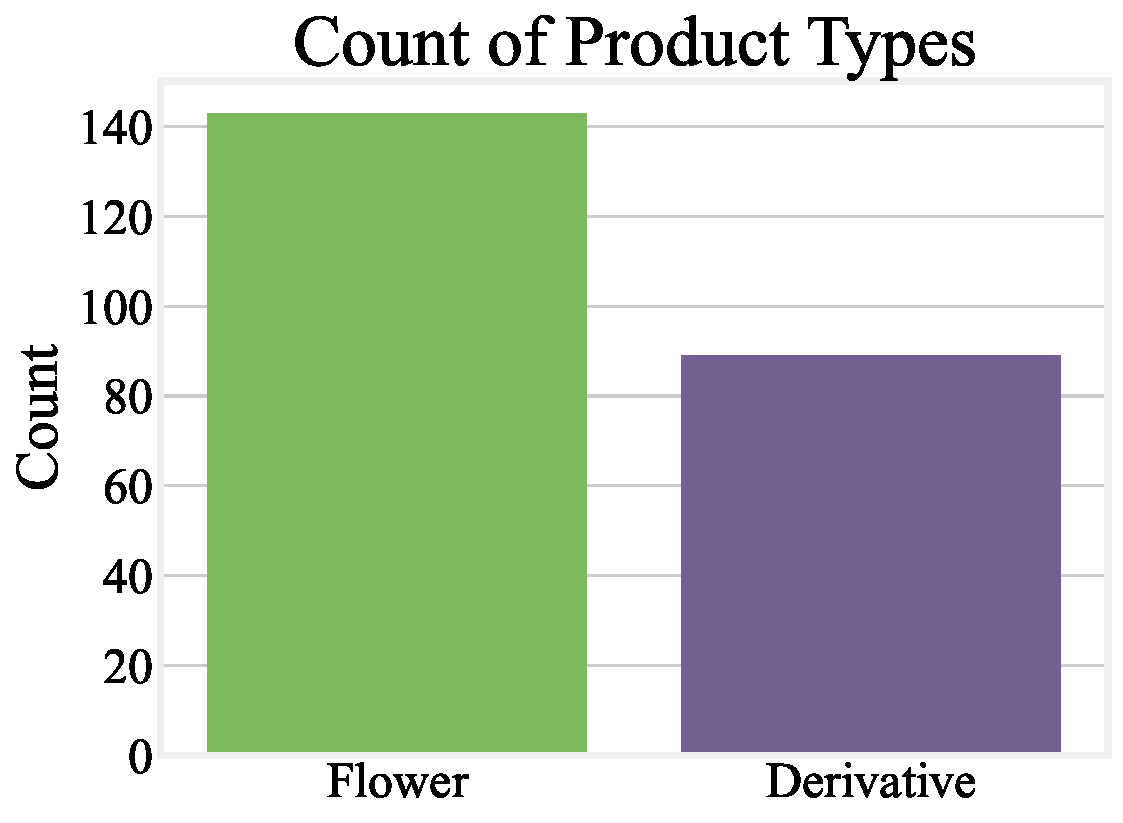
\includegraphics[width=0.4\linewidth]{figures/product-types.pdf}
\end{center}

\vspace{1\baselineskip}

% Product types pie chart.
\begin{center}
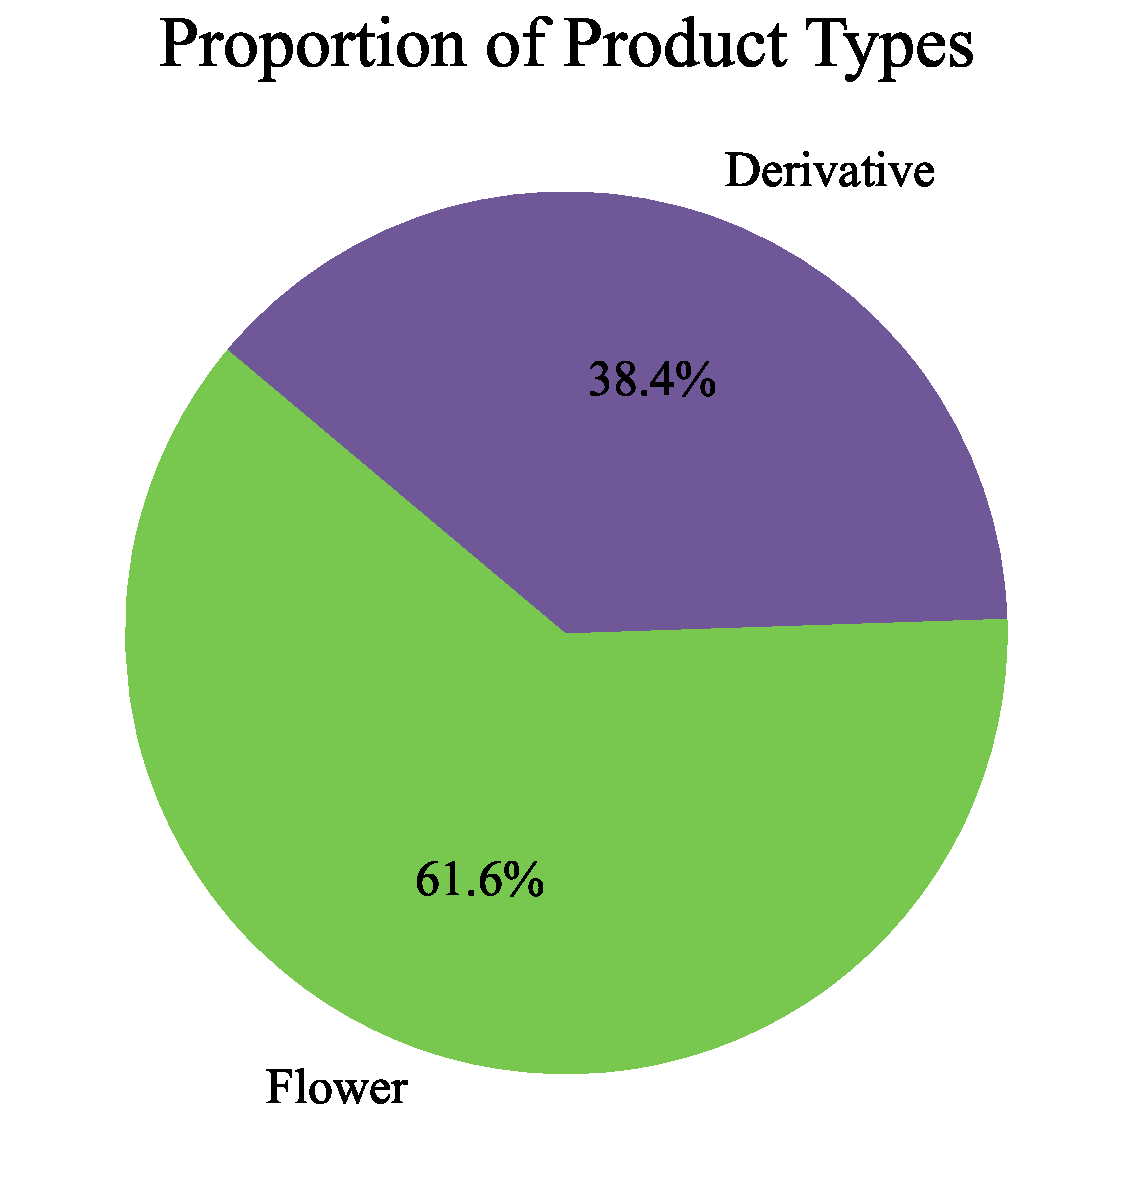
\includegraphics[width=0.4\linewidth]{figures/product-types-pie-chart.pdf}
\end{center}

%{\small
%% Strain statistics
%\begin{flushleft}
%\subfile{stats/strains}
%\end{flushleft}
%}
%


%---------------------------------%
% Chemical Analysis
%---------------------------------%
\newpage
\section*{Chemical Analysis}
\label{sec:Chemical Analysis}
\thispagestyle{regular}
%
First, we examine THCA, $\Delta$-9 THC, and CBD concentrations. We then look at the total cannabinoids and the total terpenes. Next, CBGA and other minor cannabinoids are visualized. Then, ratios of dominant terpenes are examined. We also use the Shannon Diversity Index to quantify the diversity of terpenes and cannabinoids found in each strain. Finally, PCA scores are calculated using observed dominant terpenes to create clusters of chemically similar strains.

%\vspace{1\baselineskip}
%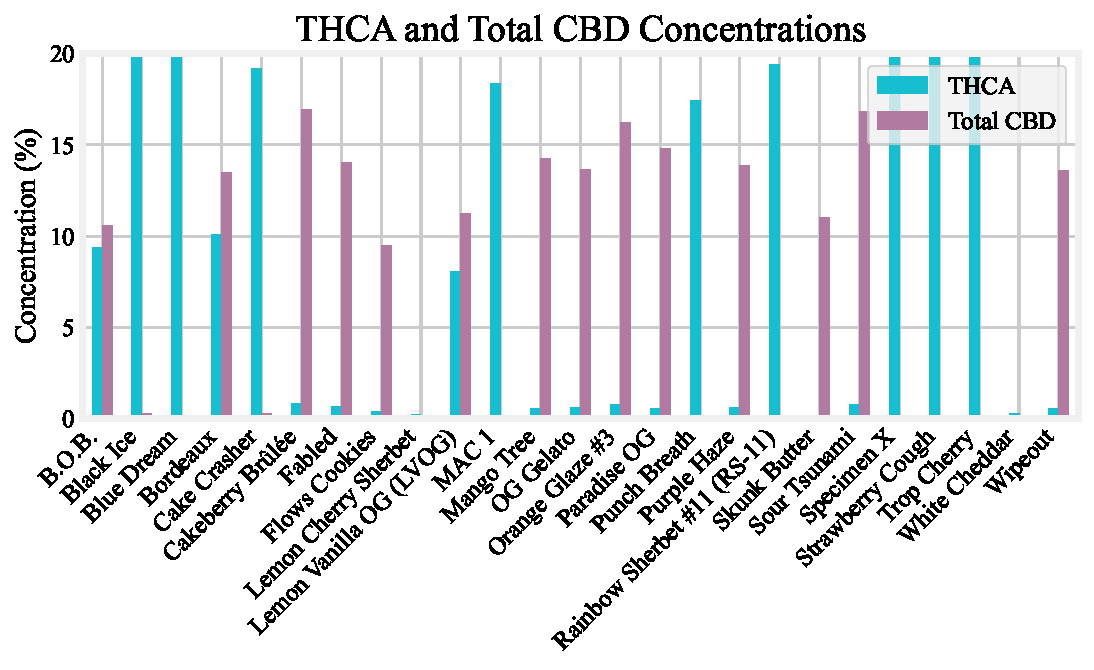
\includegraphics[width=0.95\linewidth]{figures/thca-cbd.pdf}

\vspace{1\baselineskip}

% Cannabinoid and terpene diversity bar plot.
\begin{center}
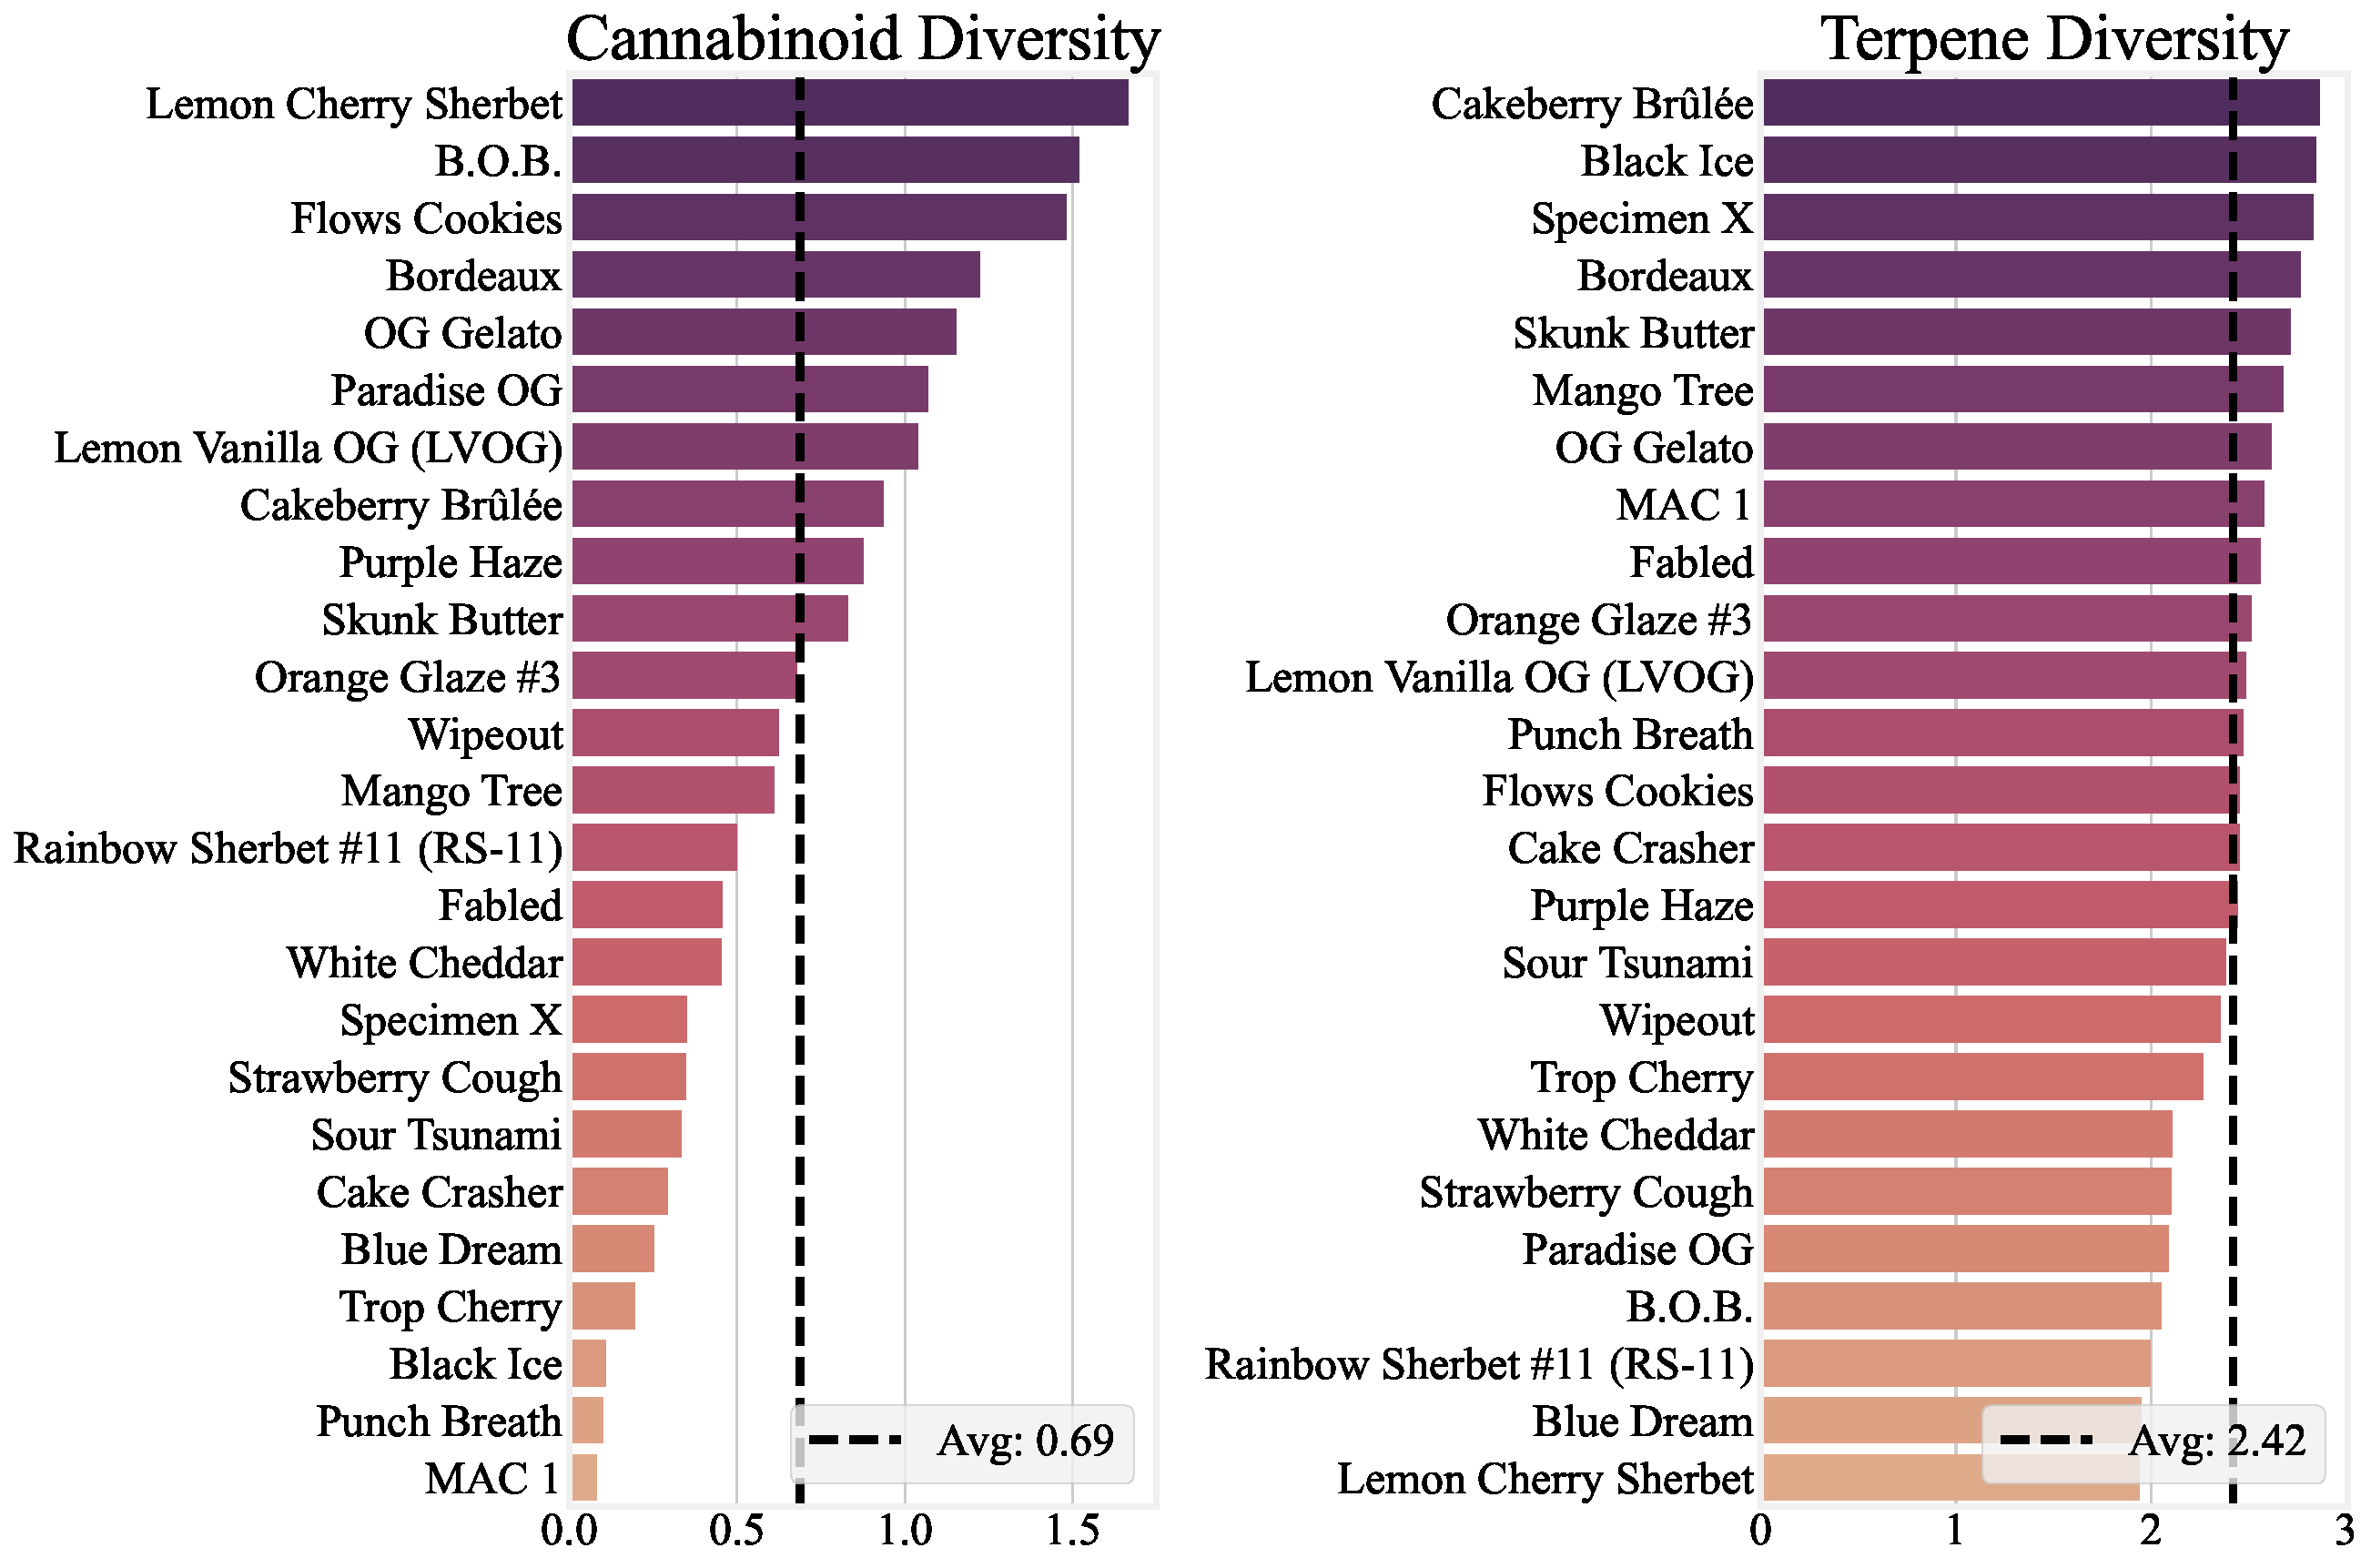
\includegraphics[width=0.875\linewidth]{figures/diversity.pdf}
\end{center}

\vspace{2\baselineskip}

% Chemical diversity scatterplot
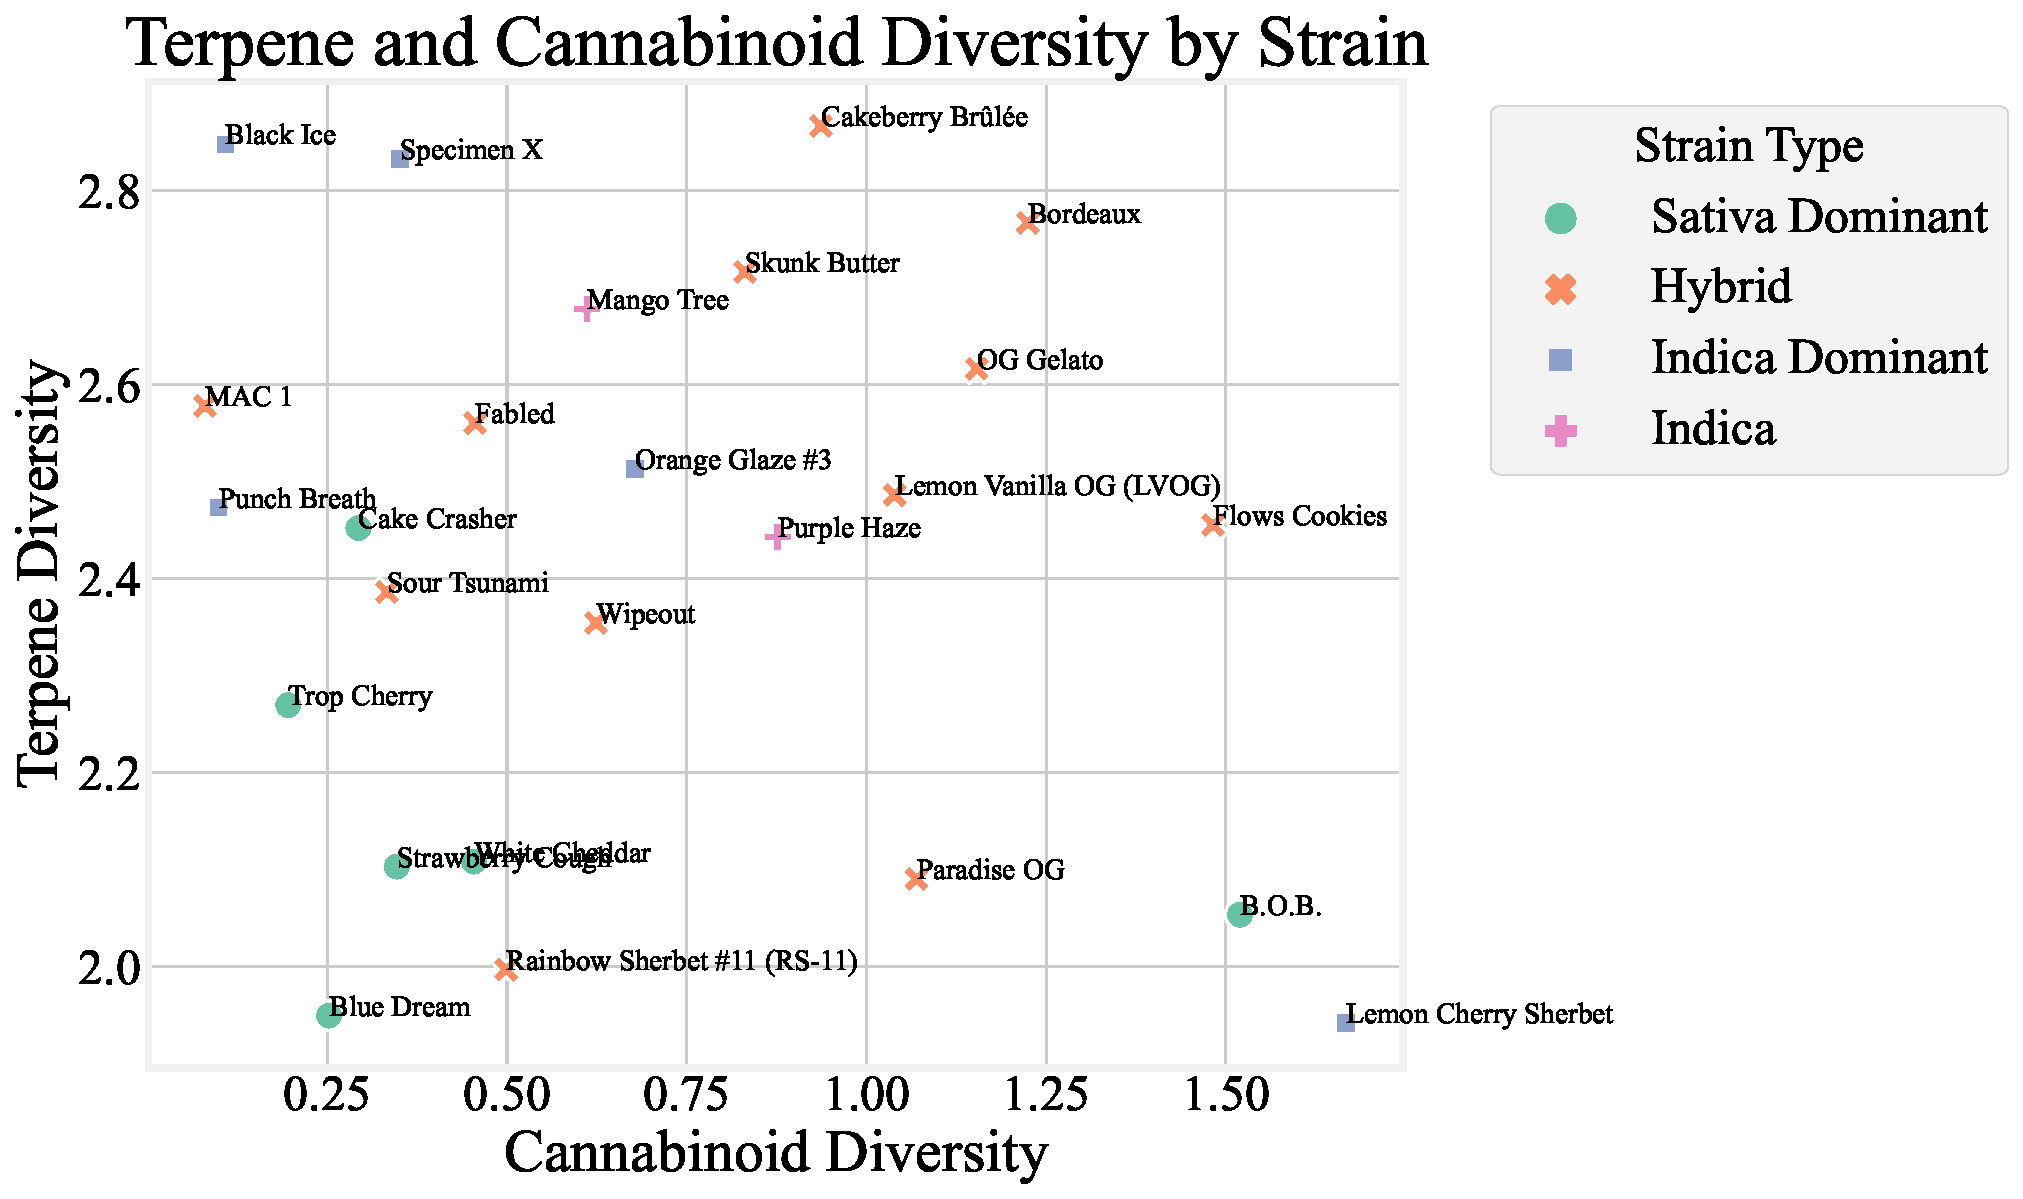
\includegraphics[width=1\linewidth]{figures/diversity-scatterplot.pdf}

\vspace{2\baselineskip}

% Compounds
{\tiny
\vspace{1\baselineskip}
\subfile{stats/compounds}
}

% Dominant terpenes.
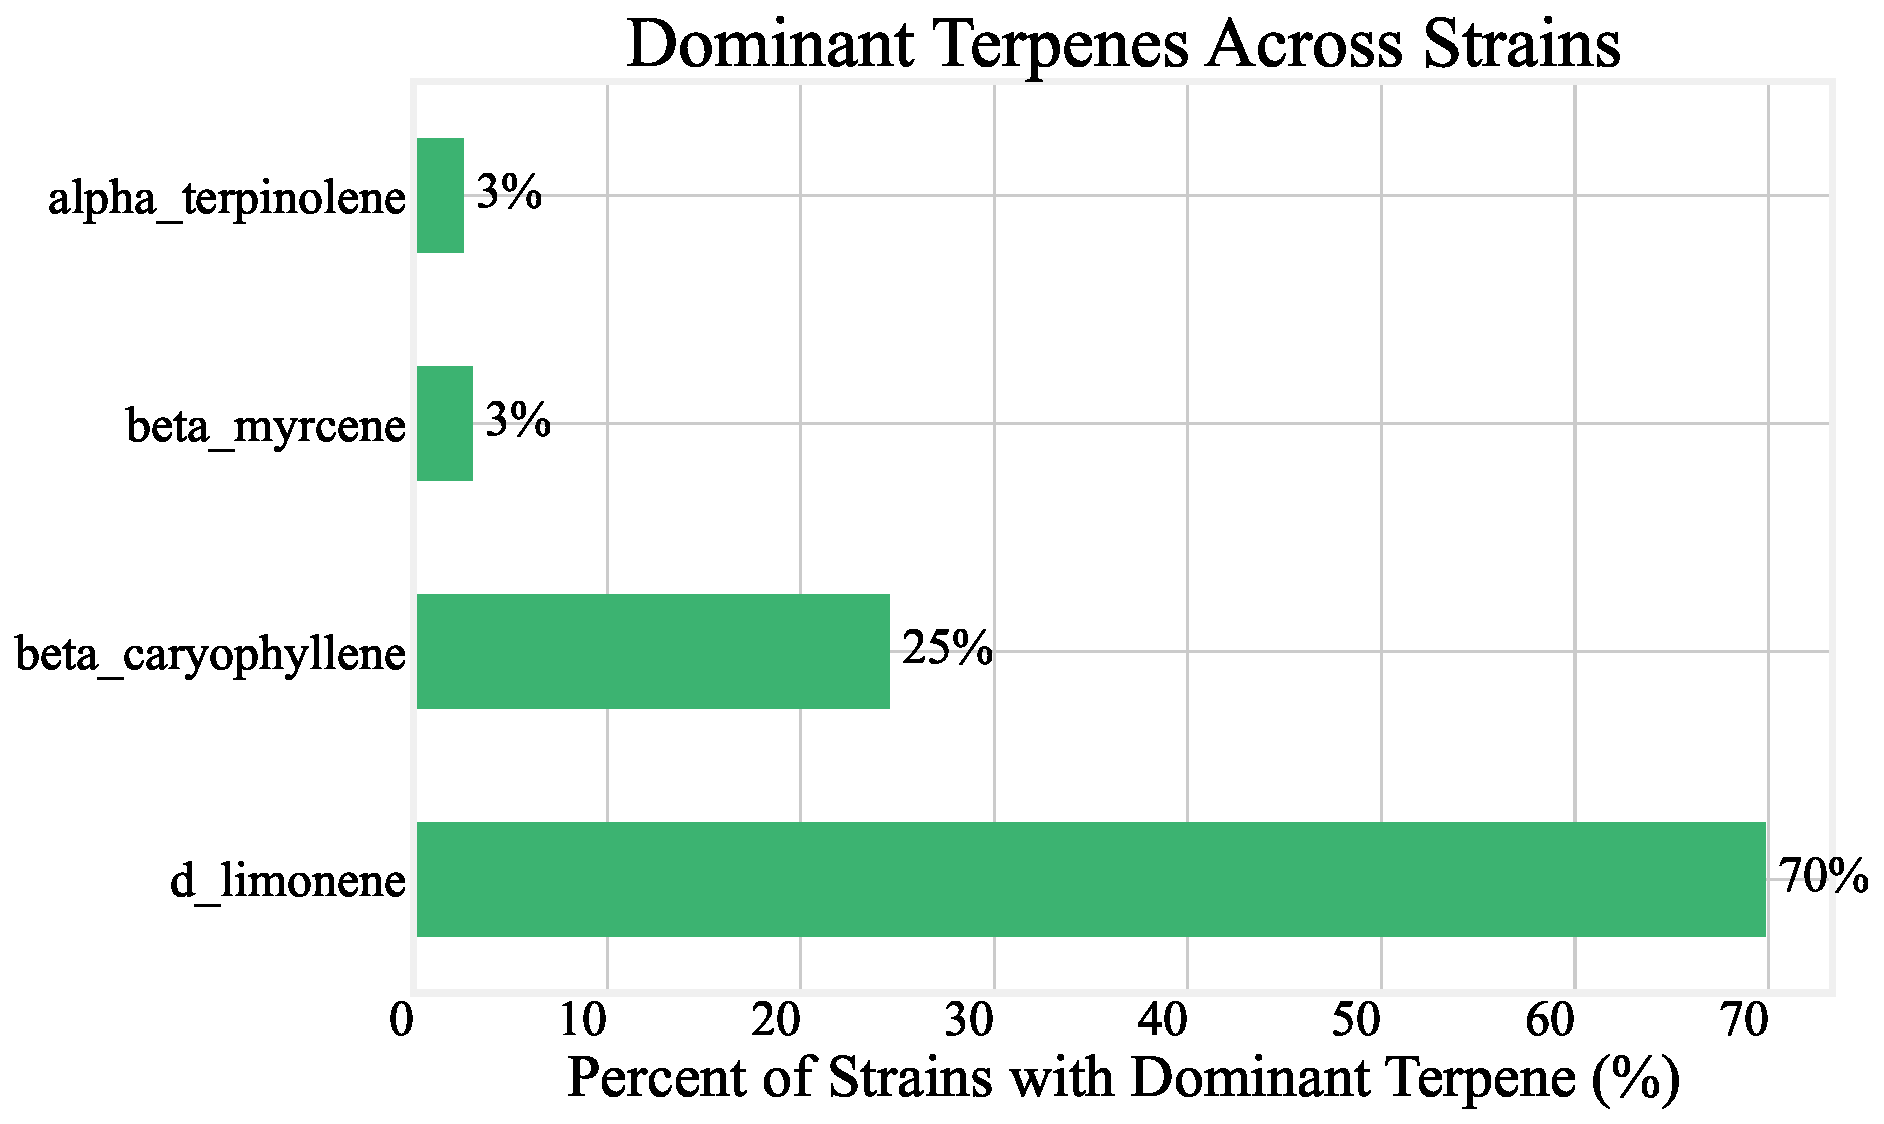
\includegraphics[width=0.95\linewidth]{figures/dominant-terpenes.pdf}

\vspace{2\baselineskip}

% Optional: Average cannabinoid profile.
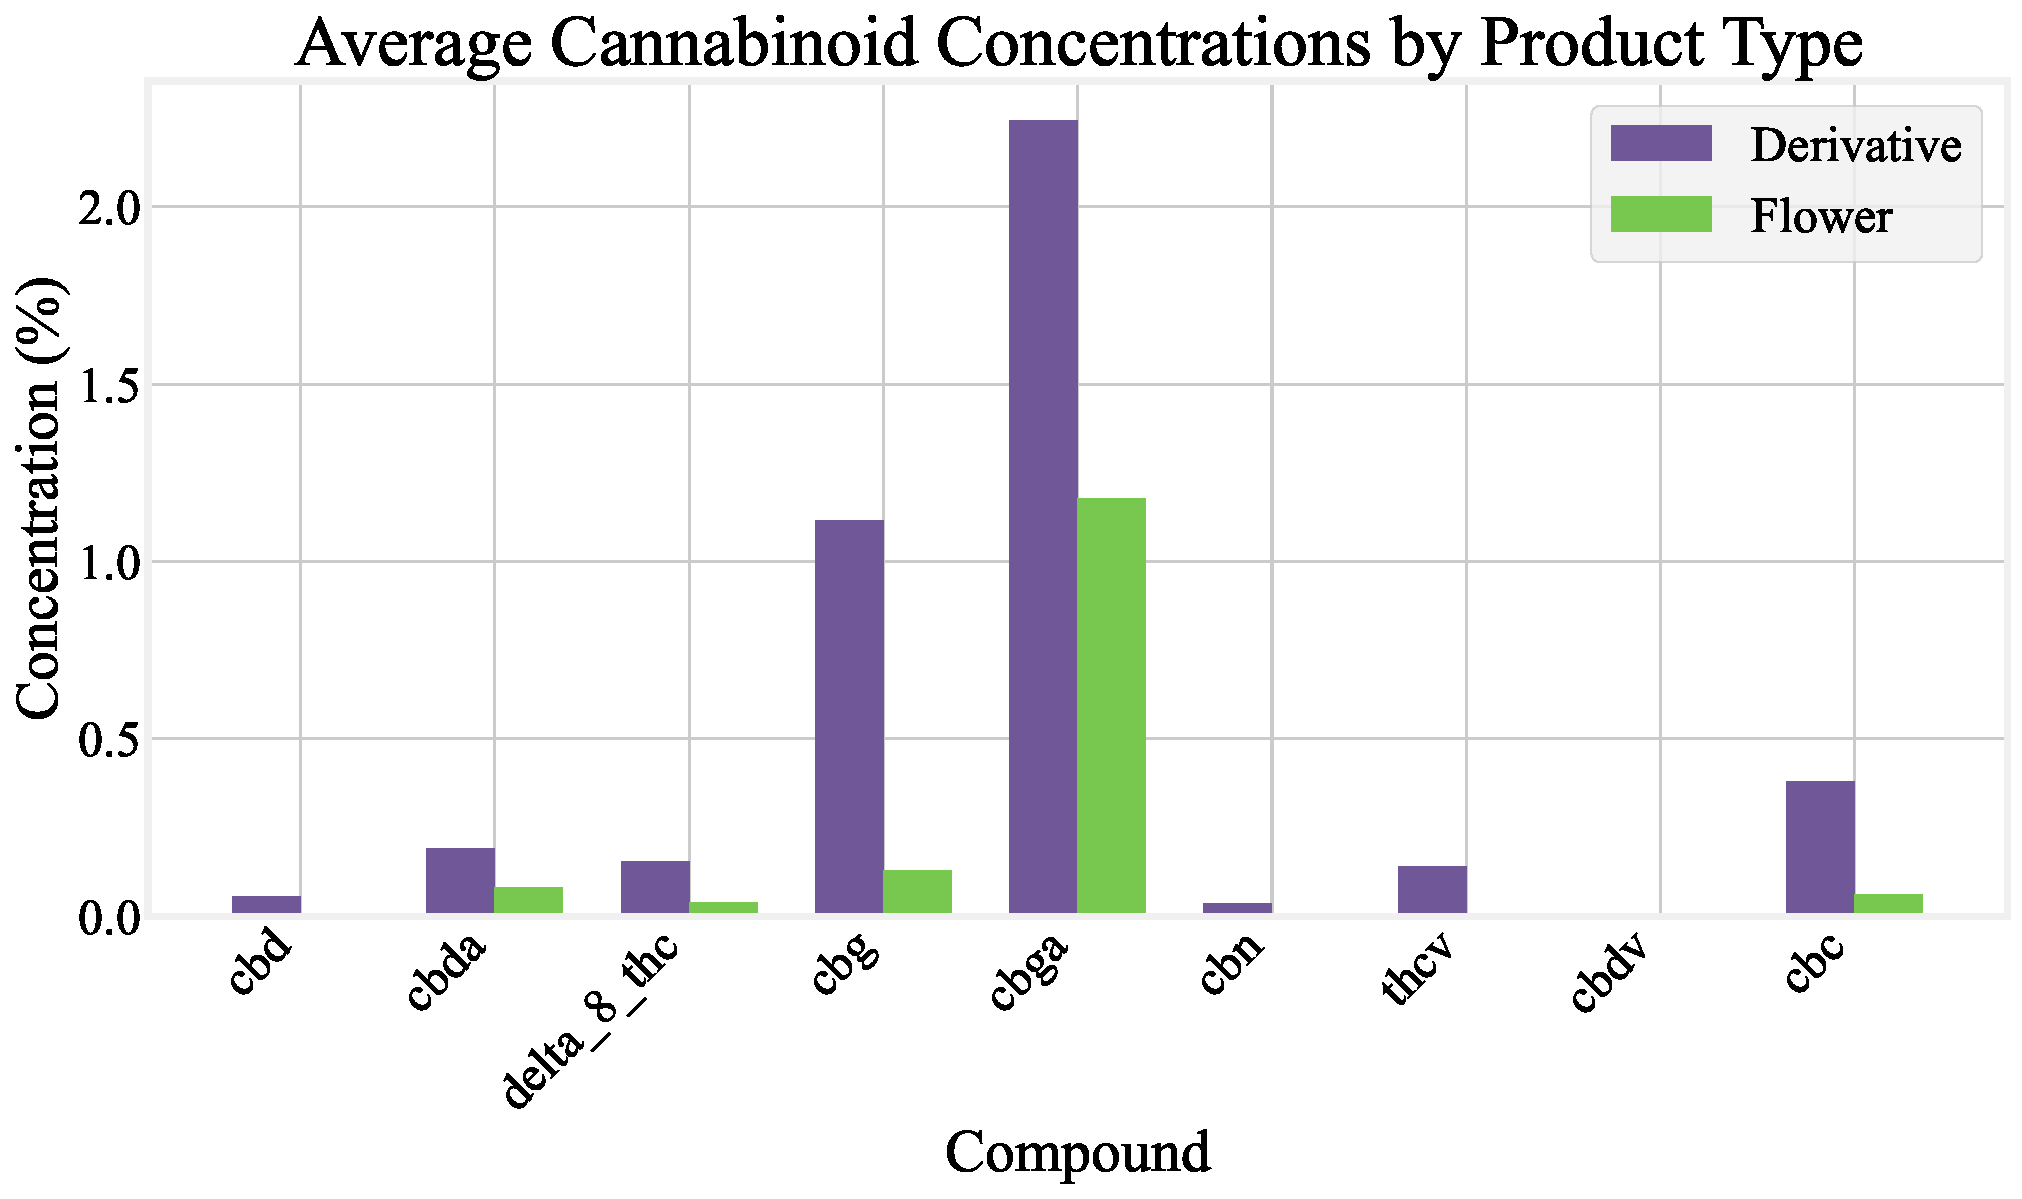
\includegraphics[width=0.95\linewidth]{figures/cannabinoids-by-type.pdf}

\vspace{2\baselineskip}

% Optional: Average terpene profile.
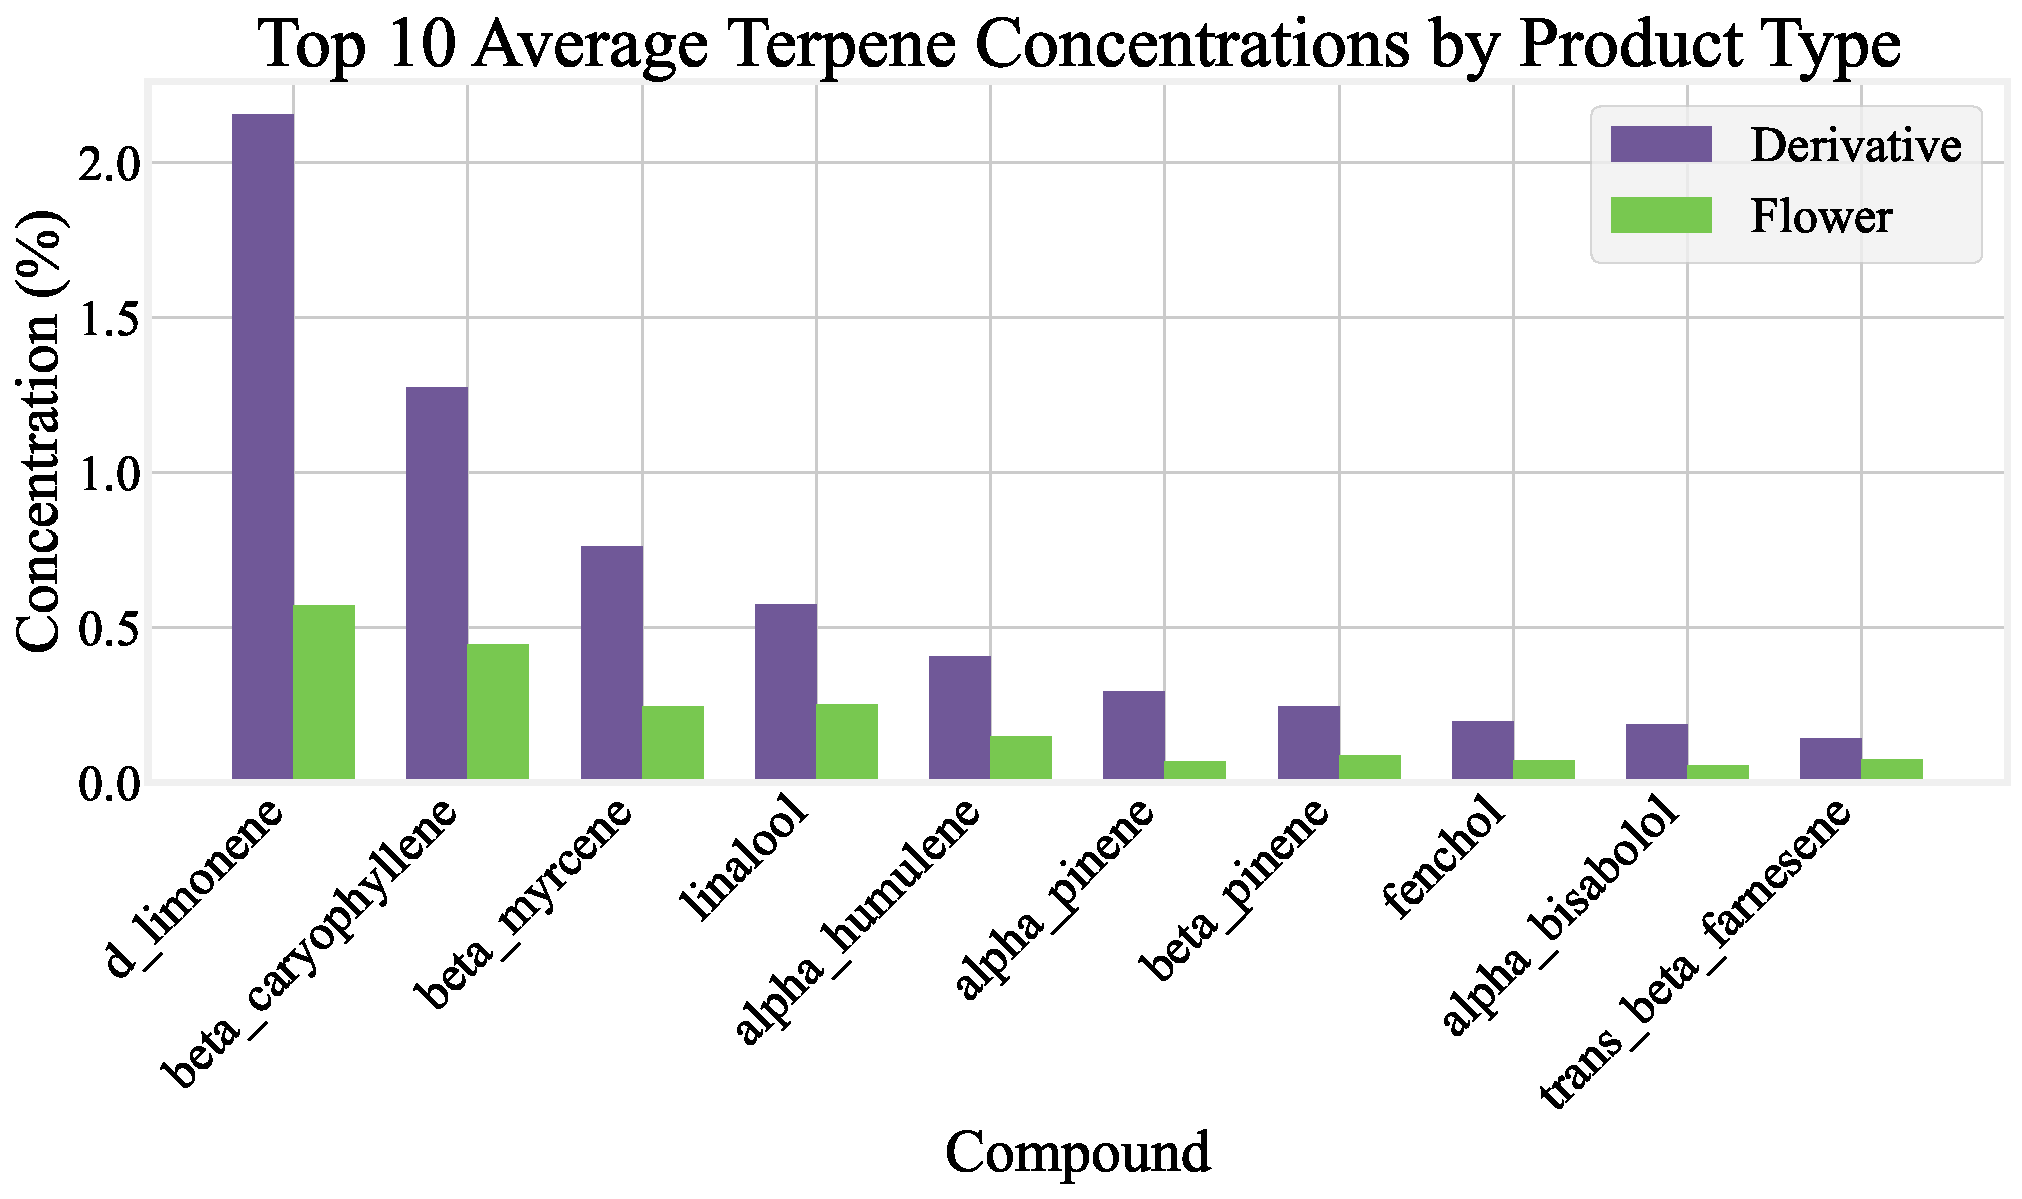
\includegraphics[width=0.95\linewidth]{figures/top-10-terpenes-by-type.pdf}

\vspace{2\baselineskip}

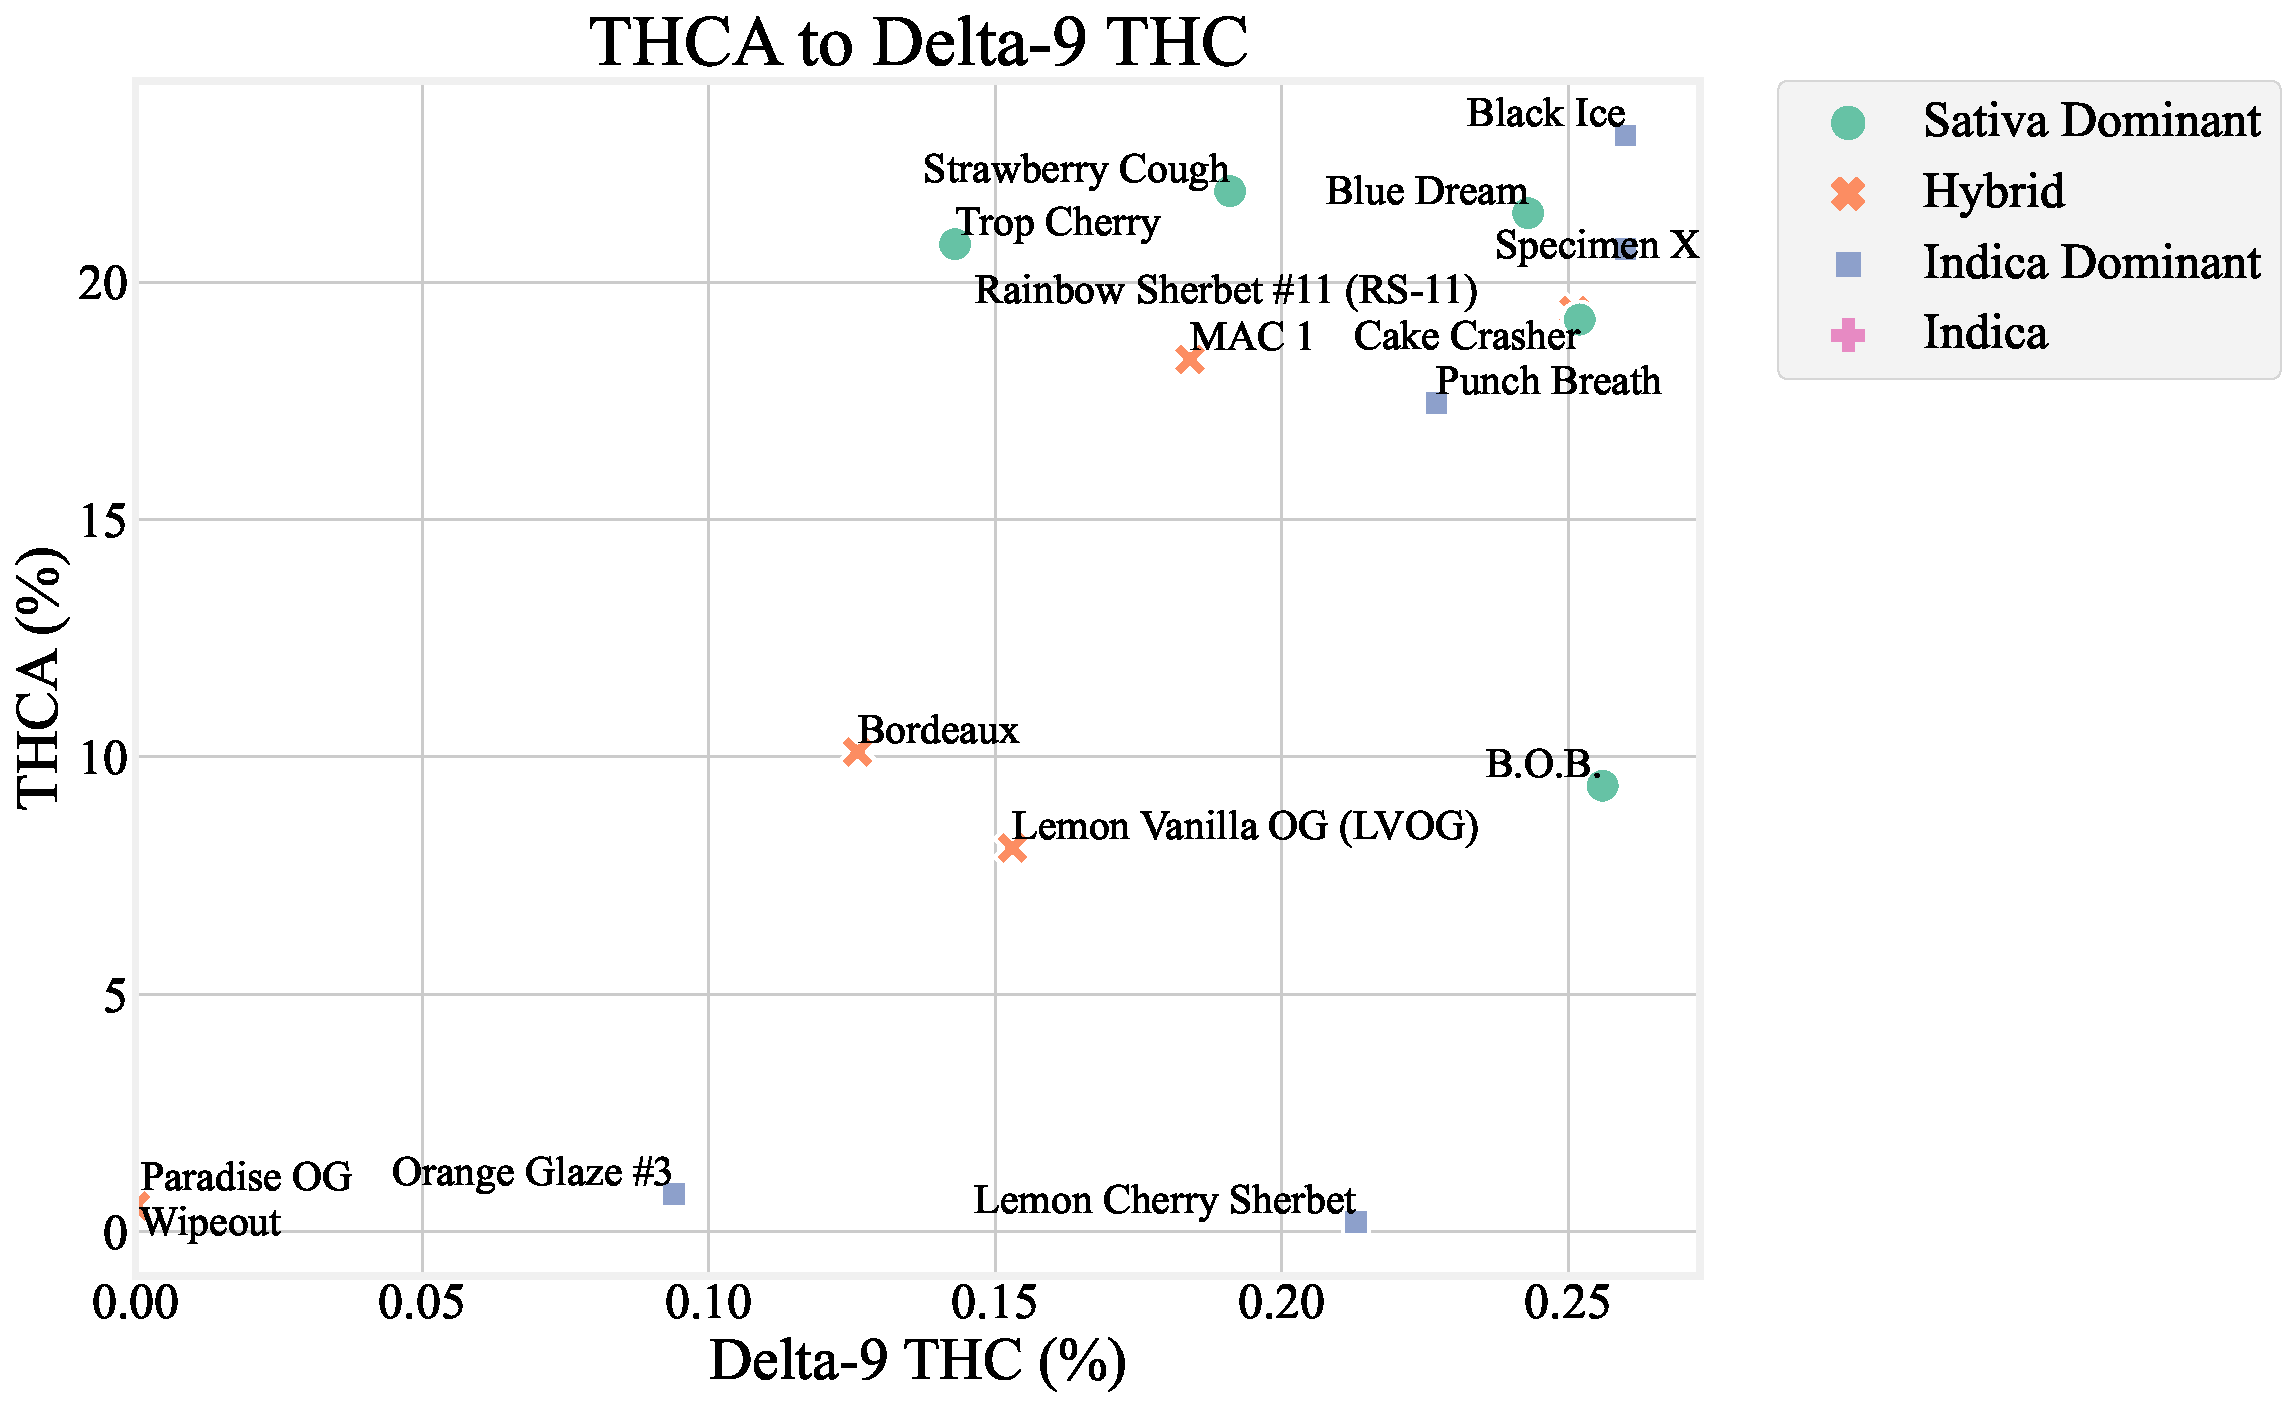
\includegraphics[width=\linewidth]{figures/thca-to-delta-9-thc.pdf}

\vspace{2\baselineskip}

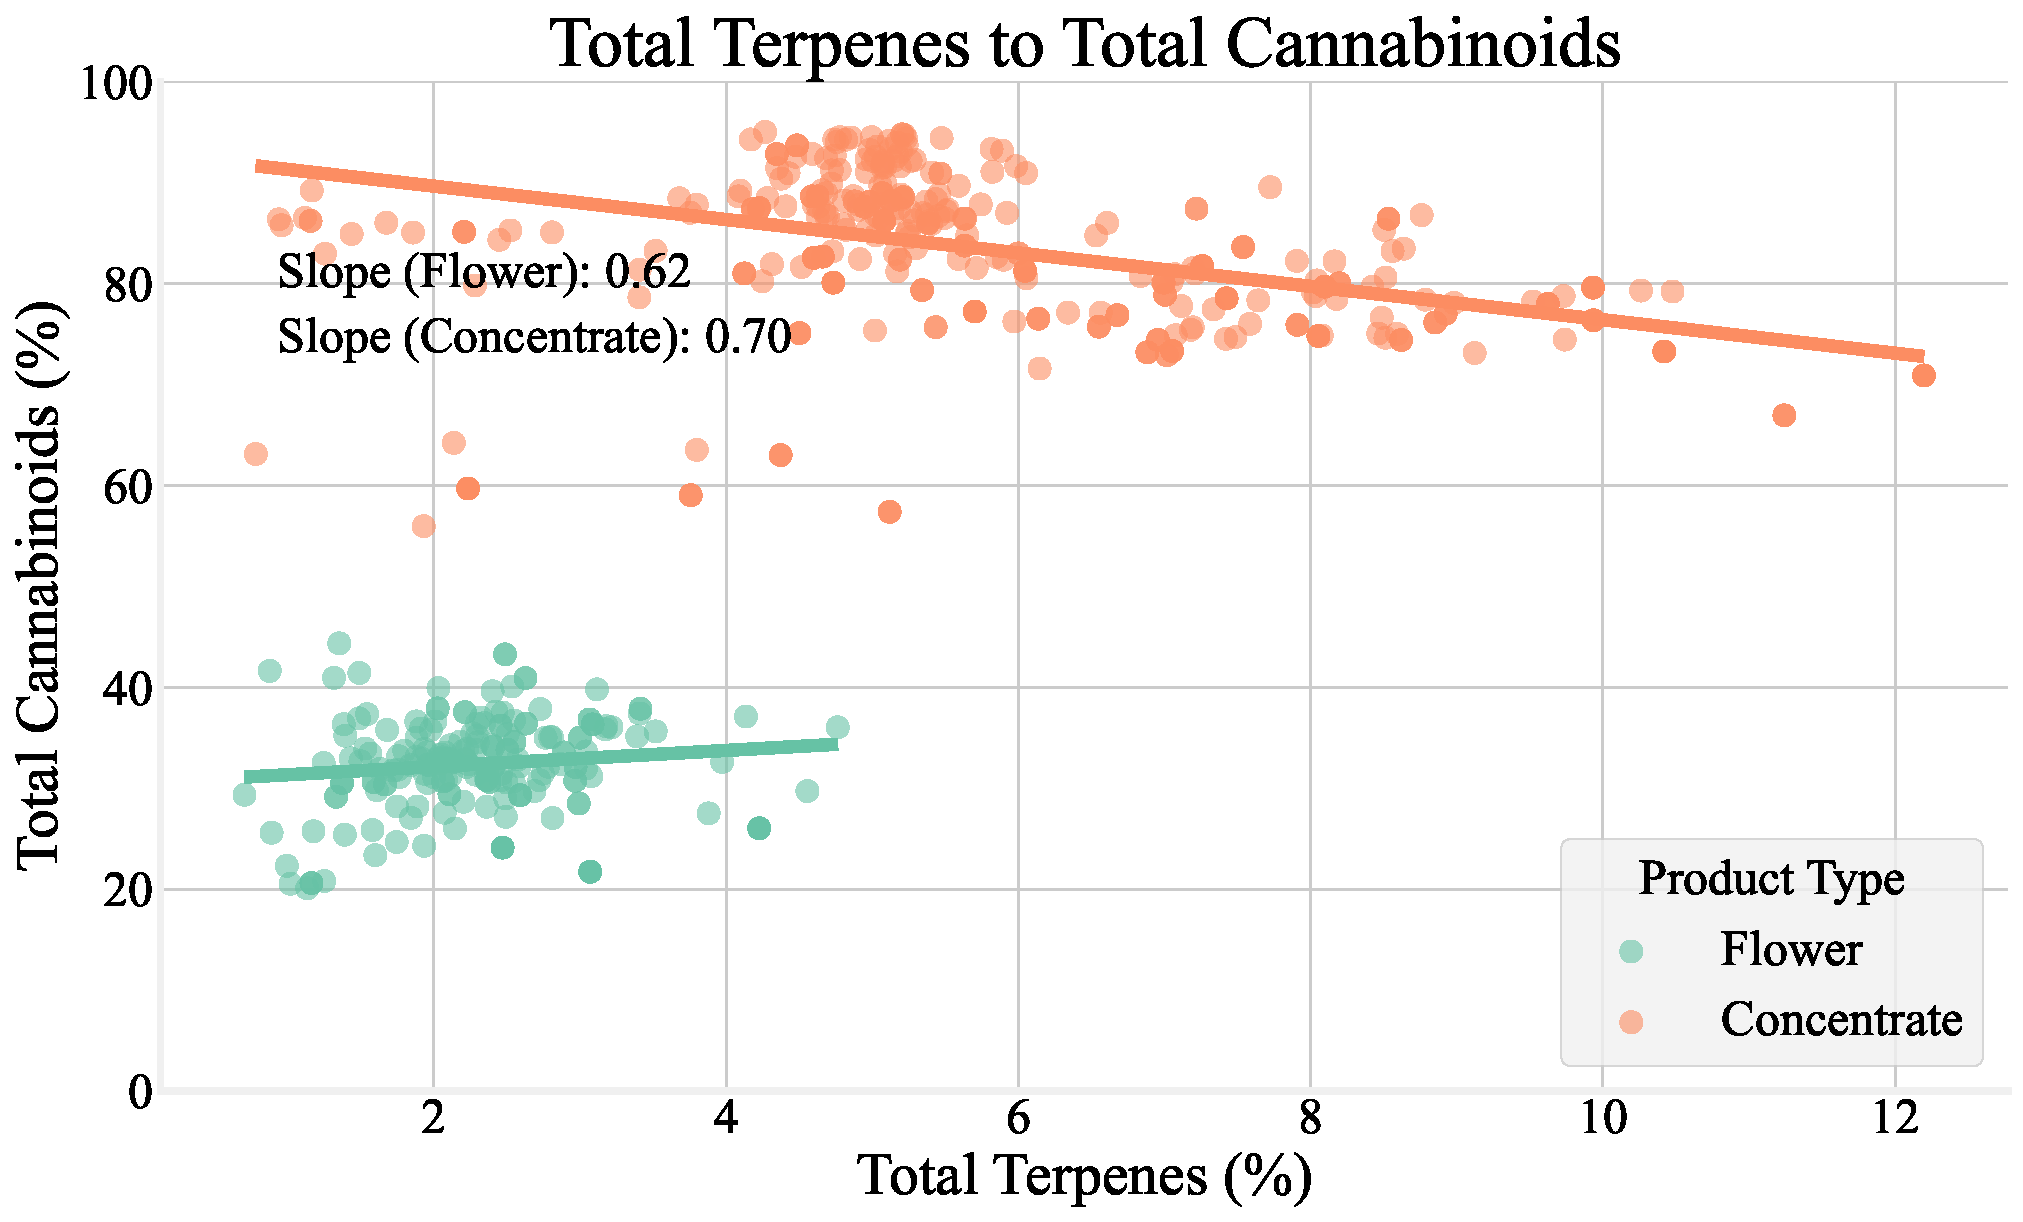
\includegraphics[width=\linewidth]{figures/total-cannabinoids-to-total-terpenes.pdf}

\vspace{2\baselineskip}

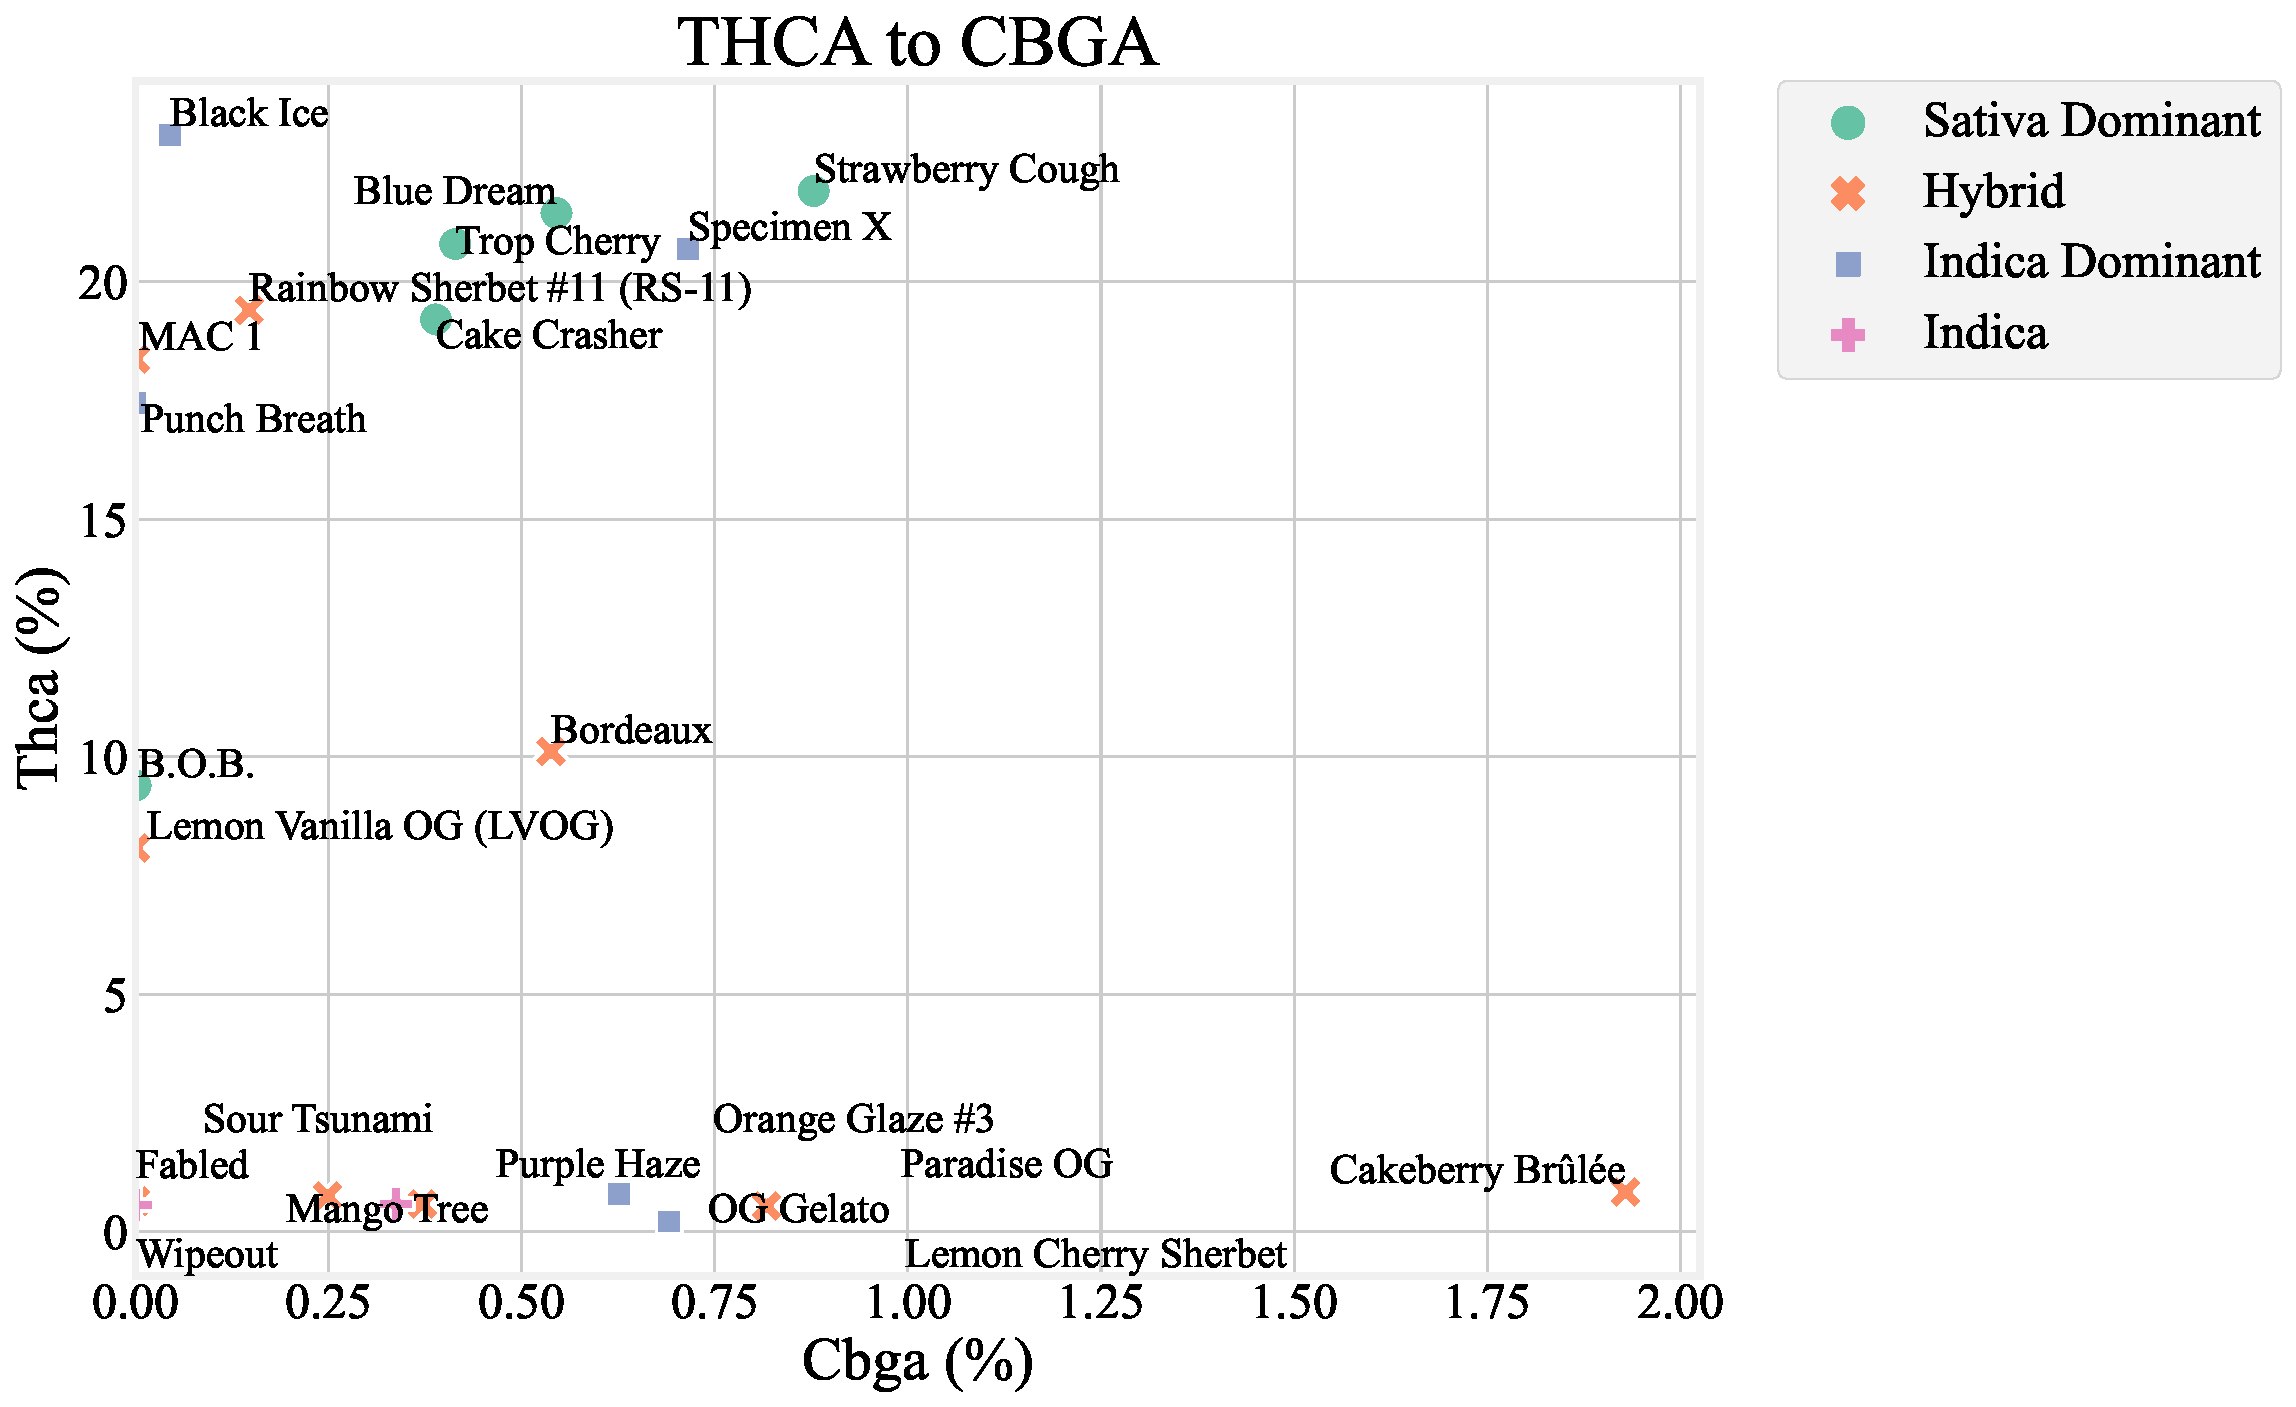
\includegraphics[width=\linewidth]{figures/thca-to-cbga.pdf}

\vspace{2\baselineskip}

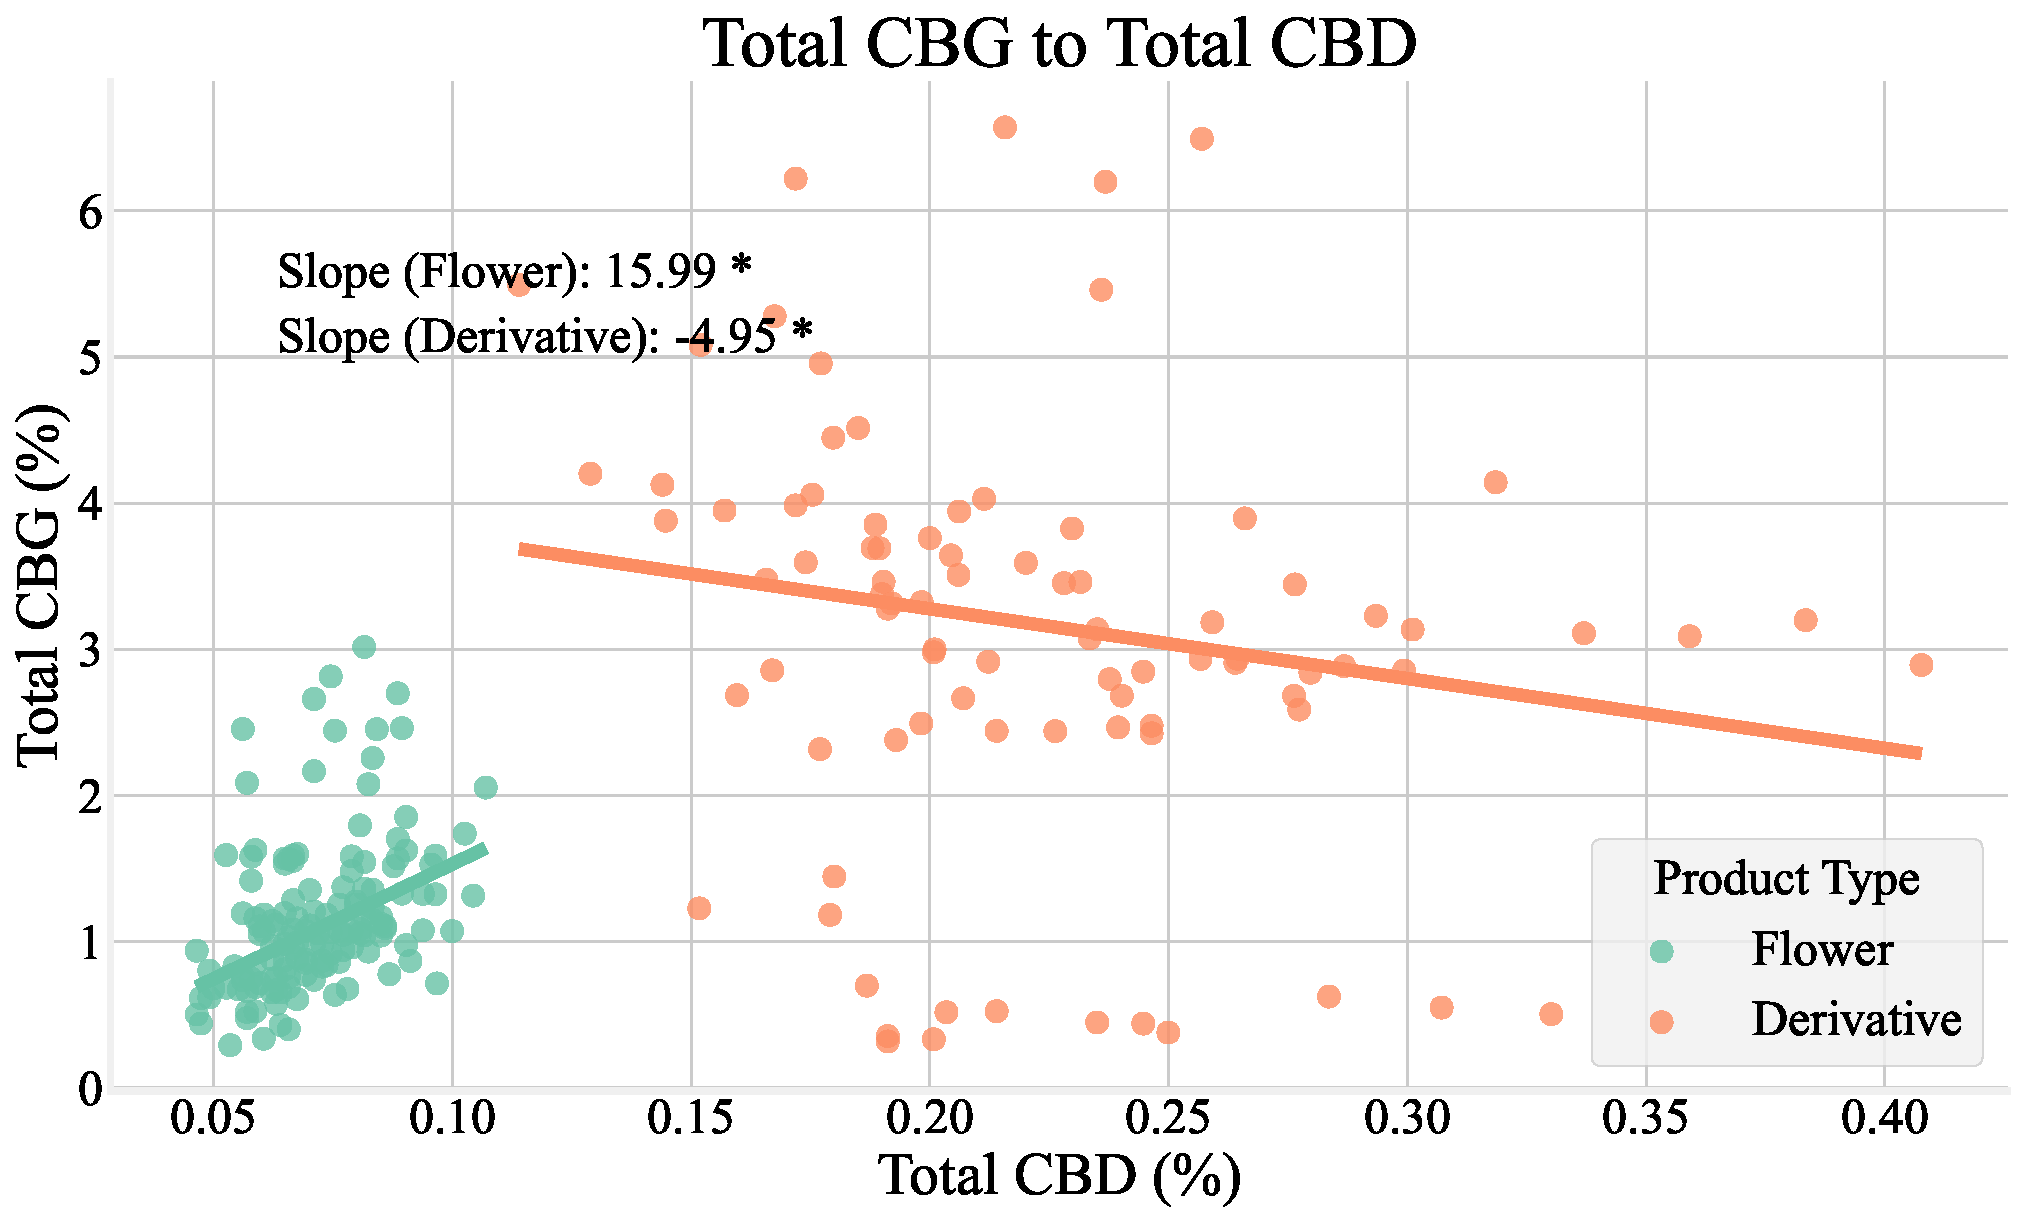
\includegraphics[width=\linewidth]{figures/total-cbg-to-calculated-total-cbd.pdf}

\vspace{2\baselineskip}

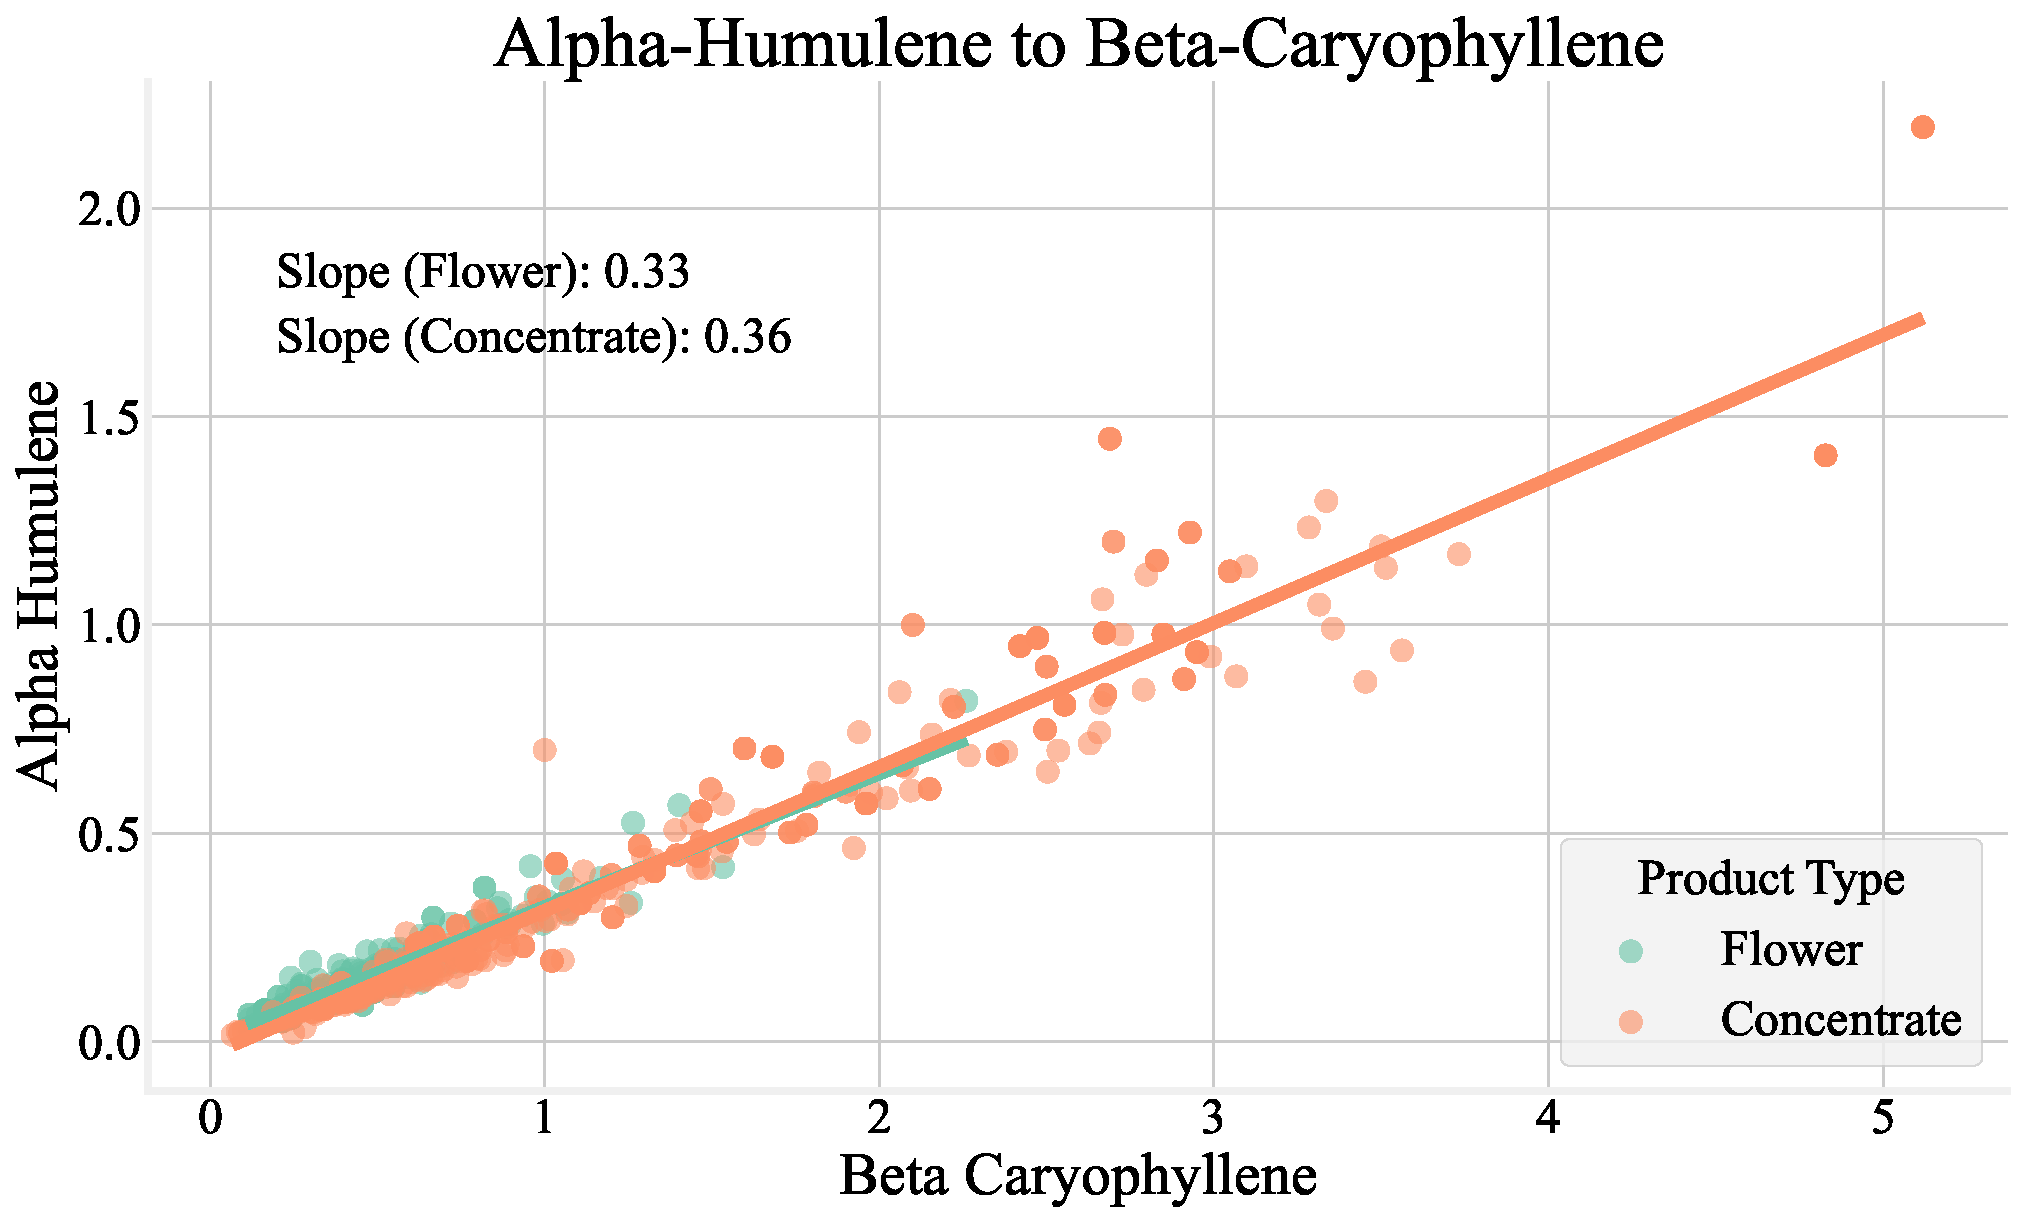
\includegraphics[width=\linewidth]{figures/alpha-humulene-to-beta-caryophyllene.pdf}

\vspace{2\baselineskip}

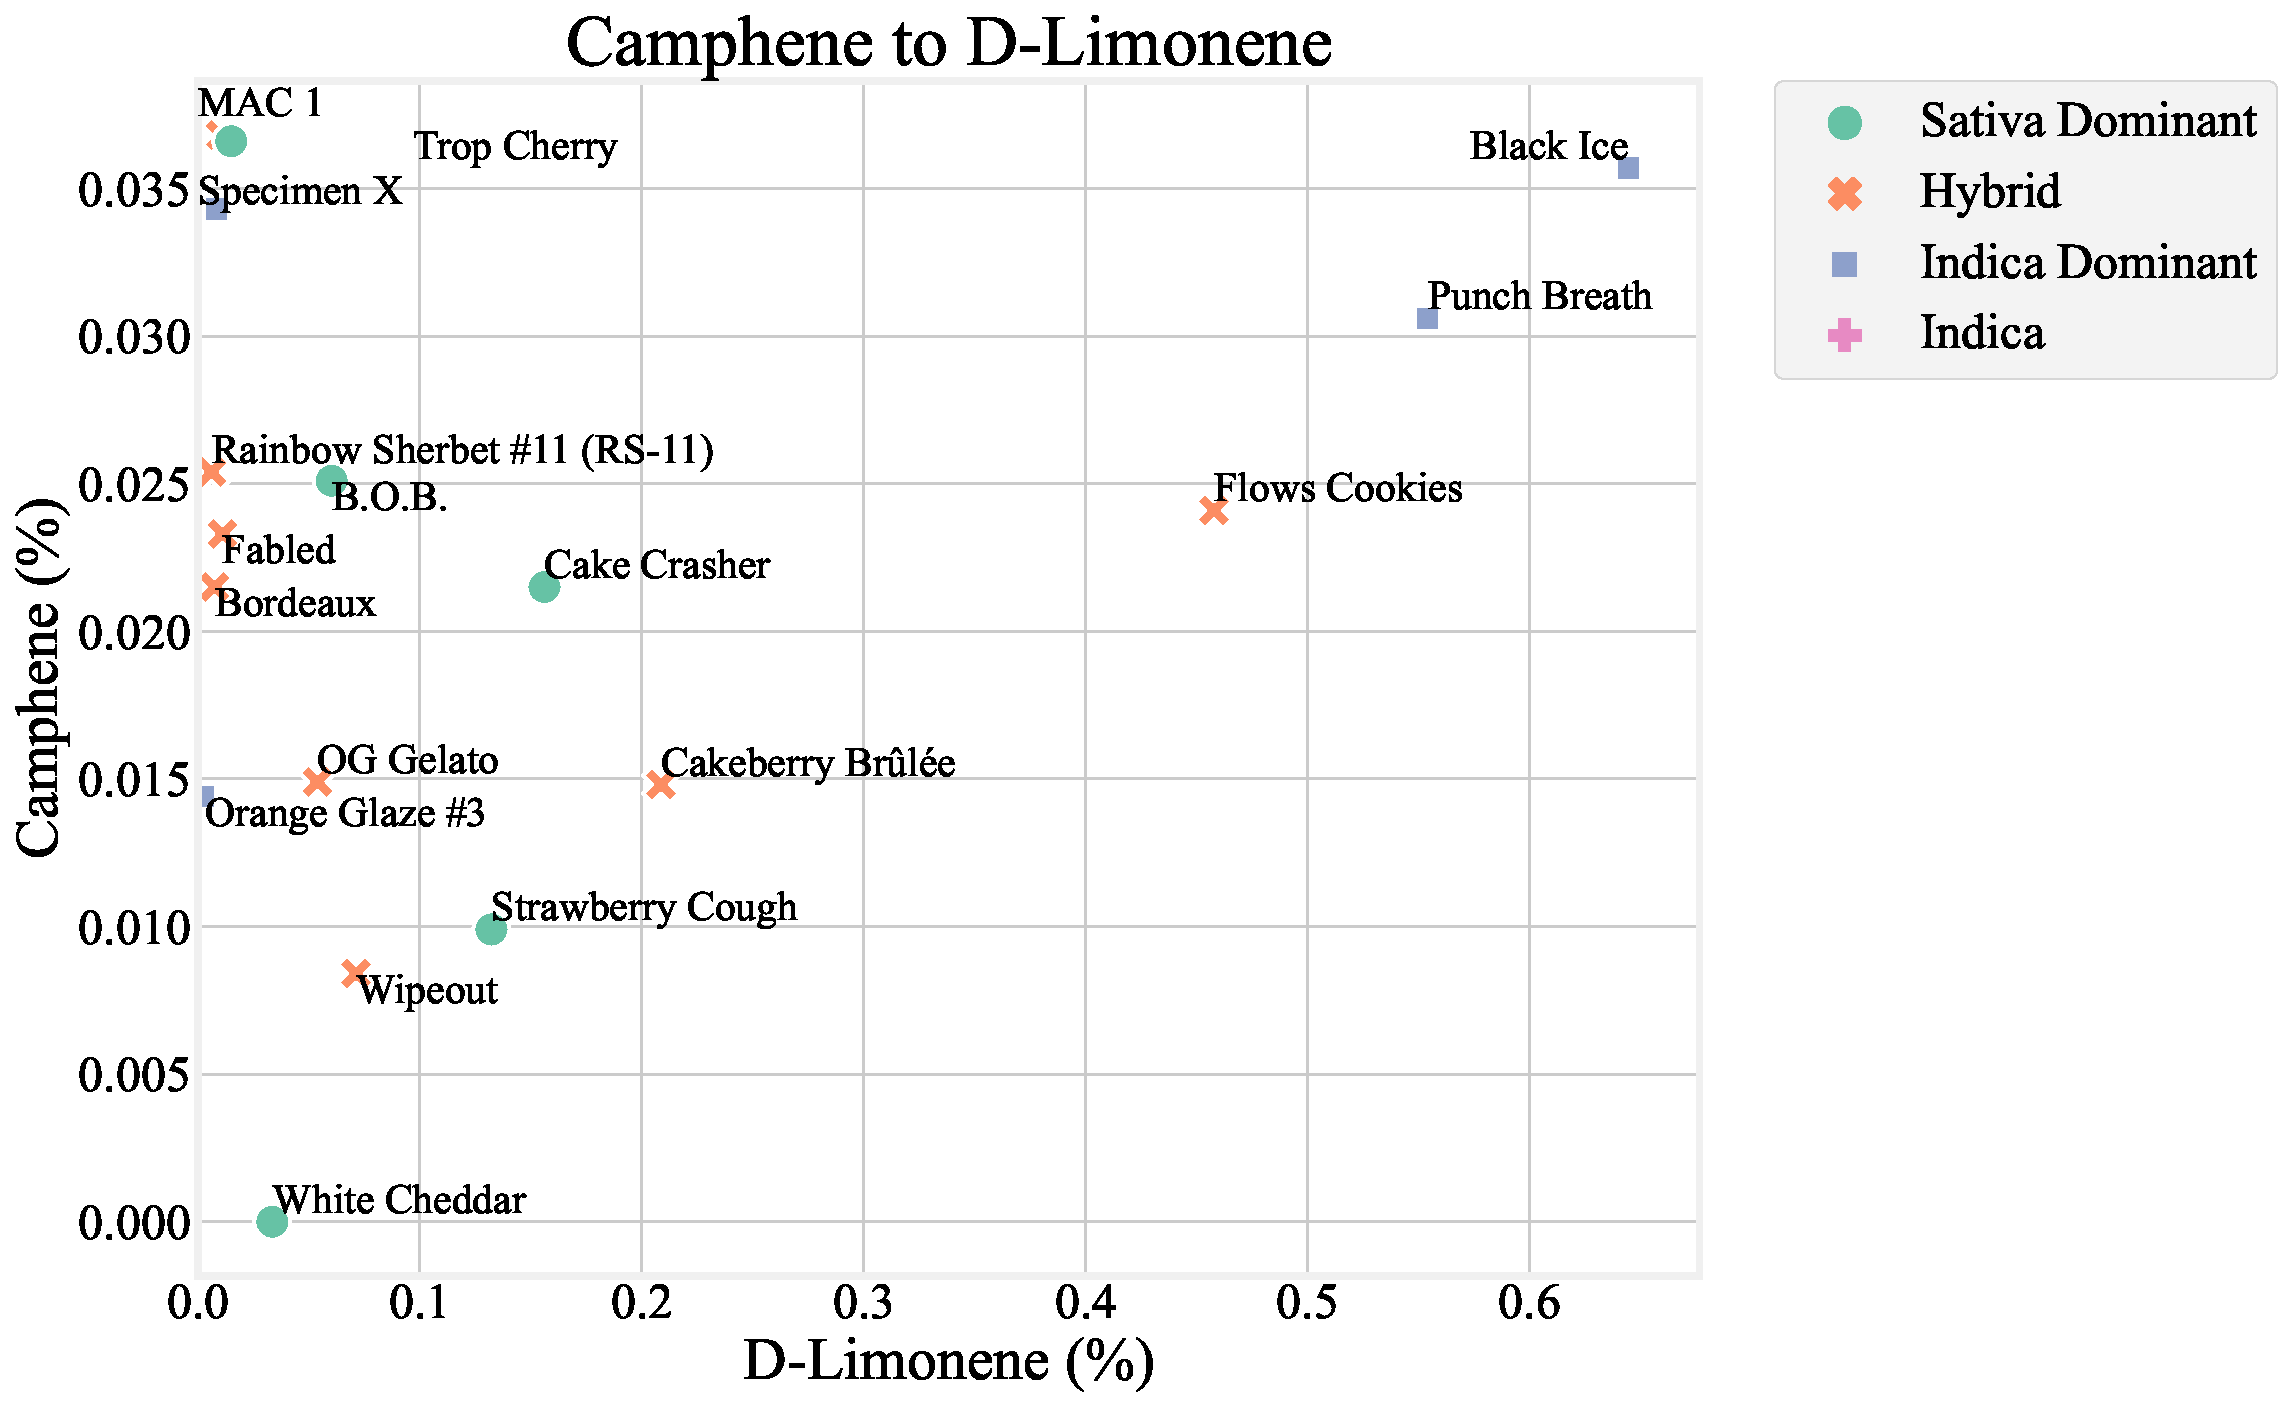
\includegraphics[width=\linewidth]{figures/camphene-to-d-limonene.pdf}

\vspace{2\baselineskip}

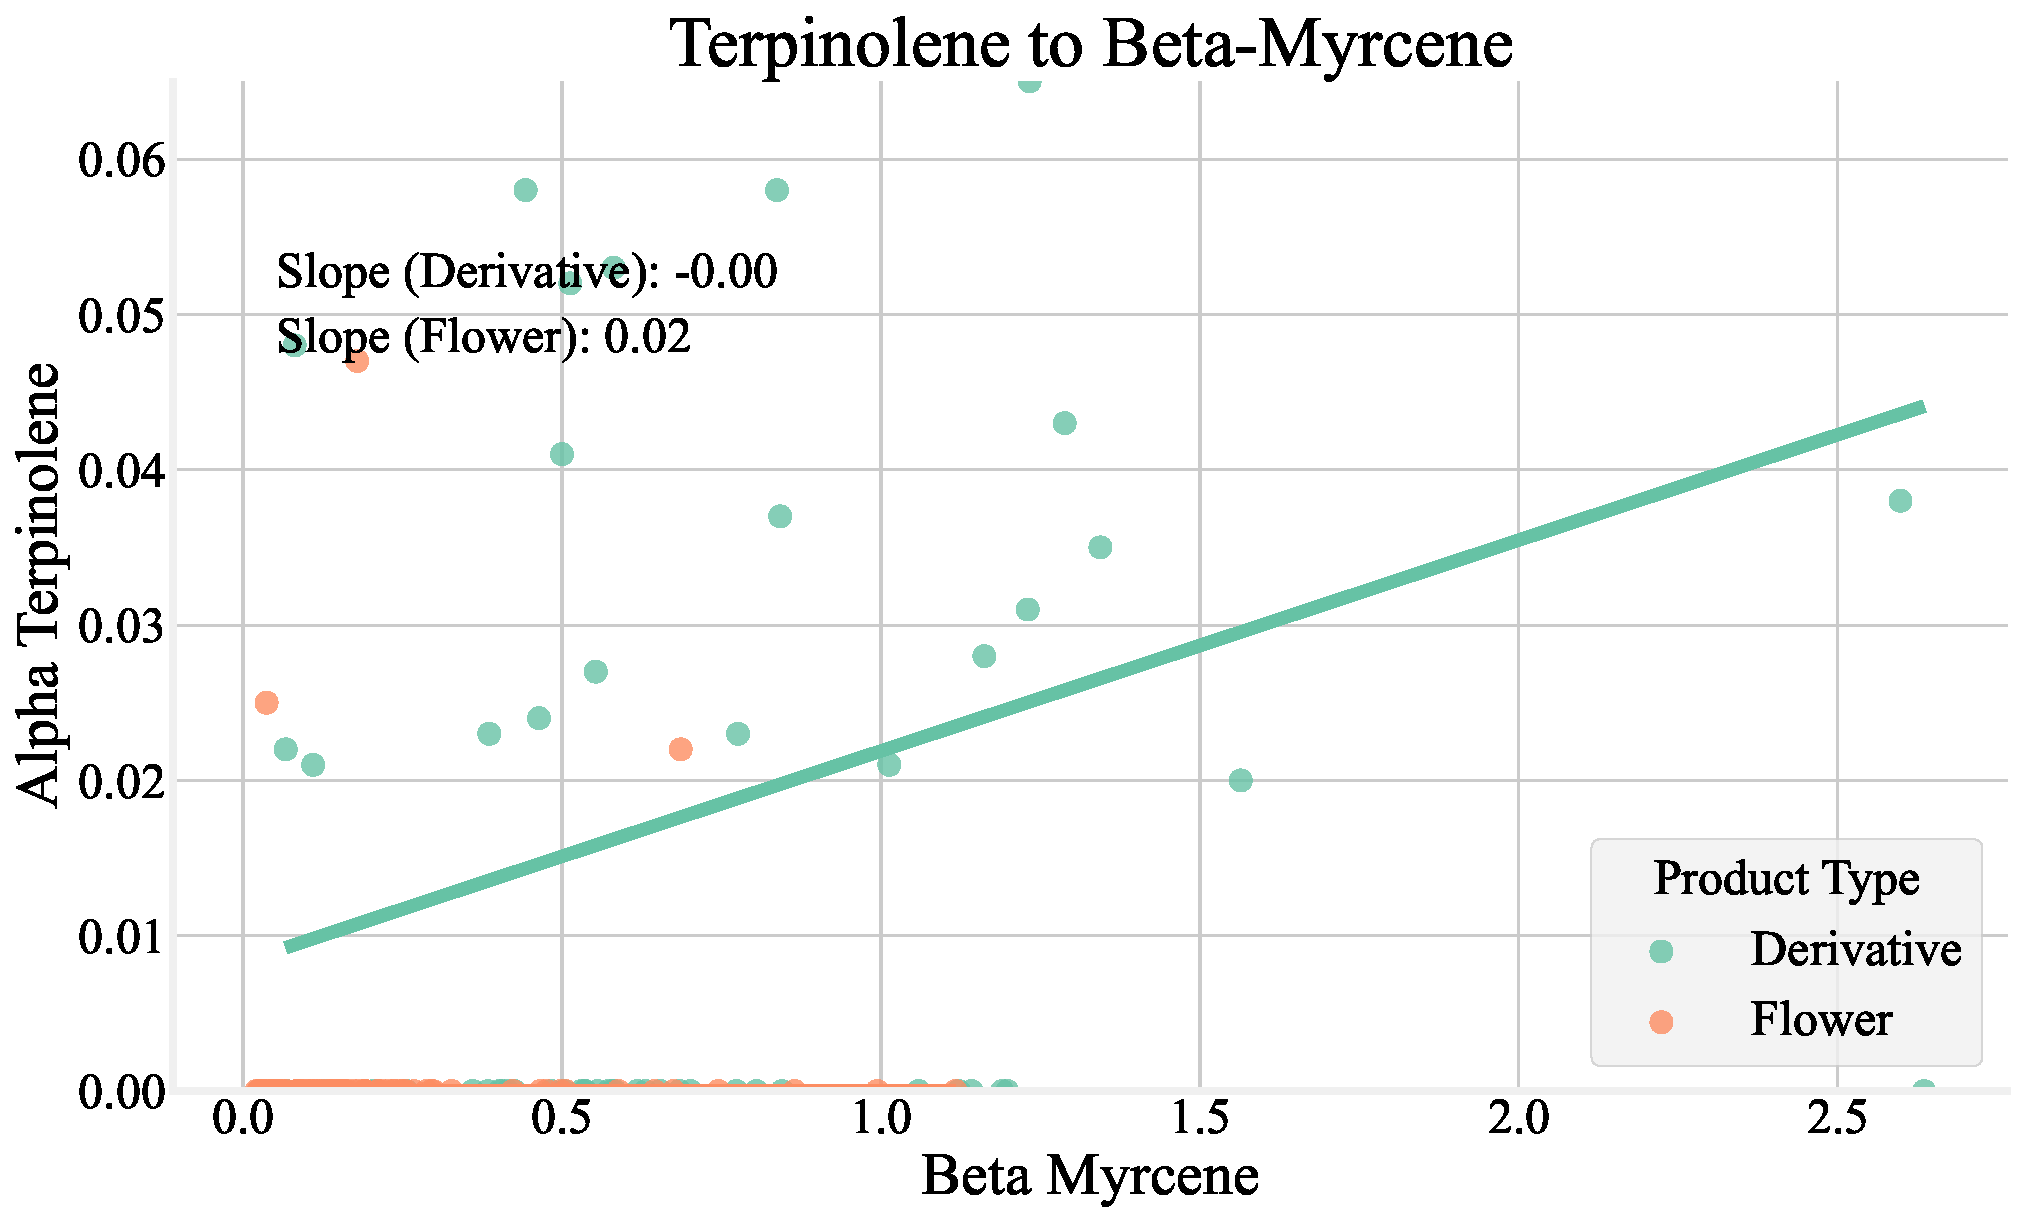
\includegraphics[width=\linewidth]{figures/alpha-terpinolene-to-beta-myrcene.pdf}

\vspace{2\baselineskip}

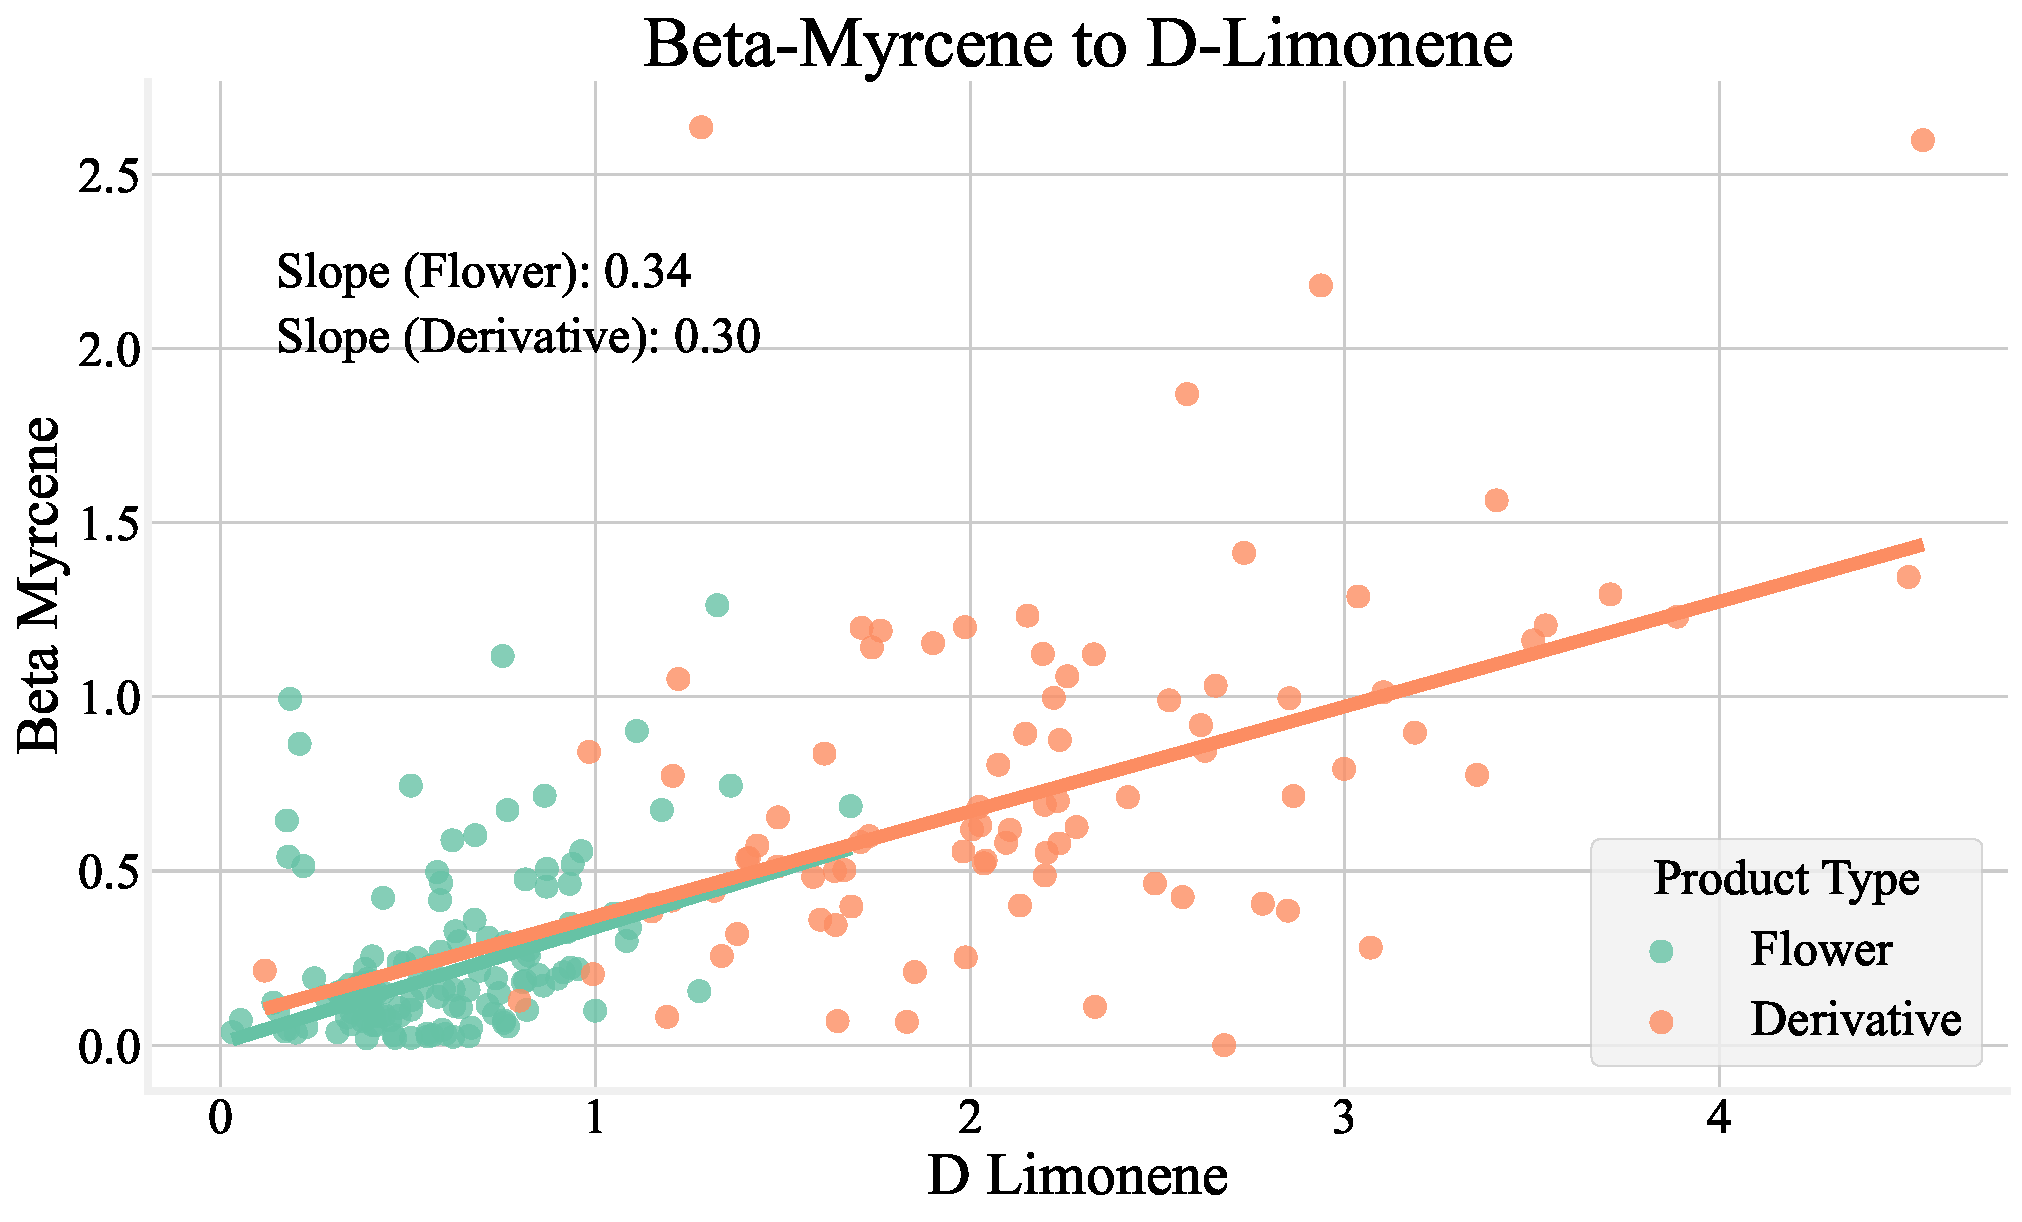
\includegraphics[width=\linewidth]{figures/beta-myrcene-to-d-limonene.pdf}

\vspace{2\baselineskip}

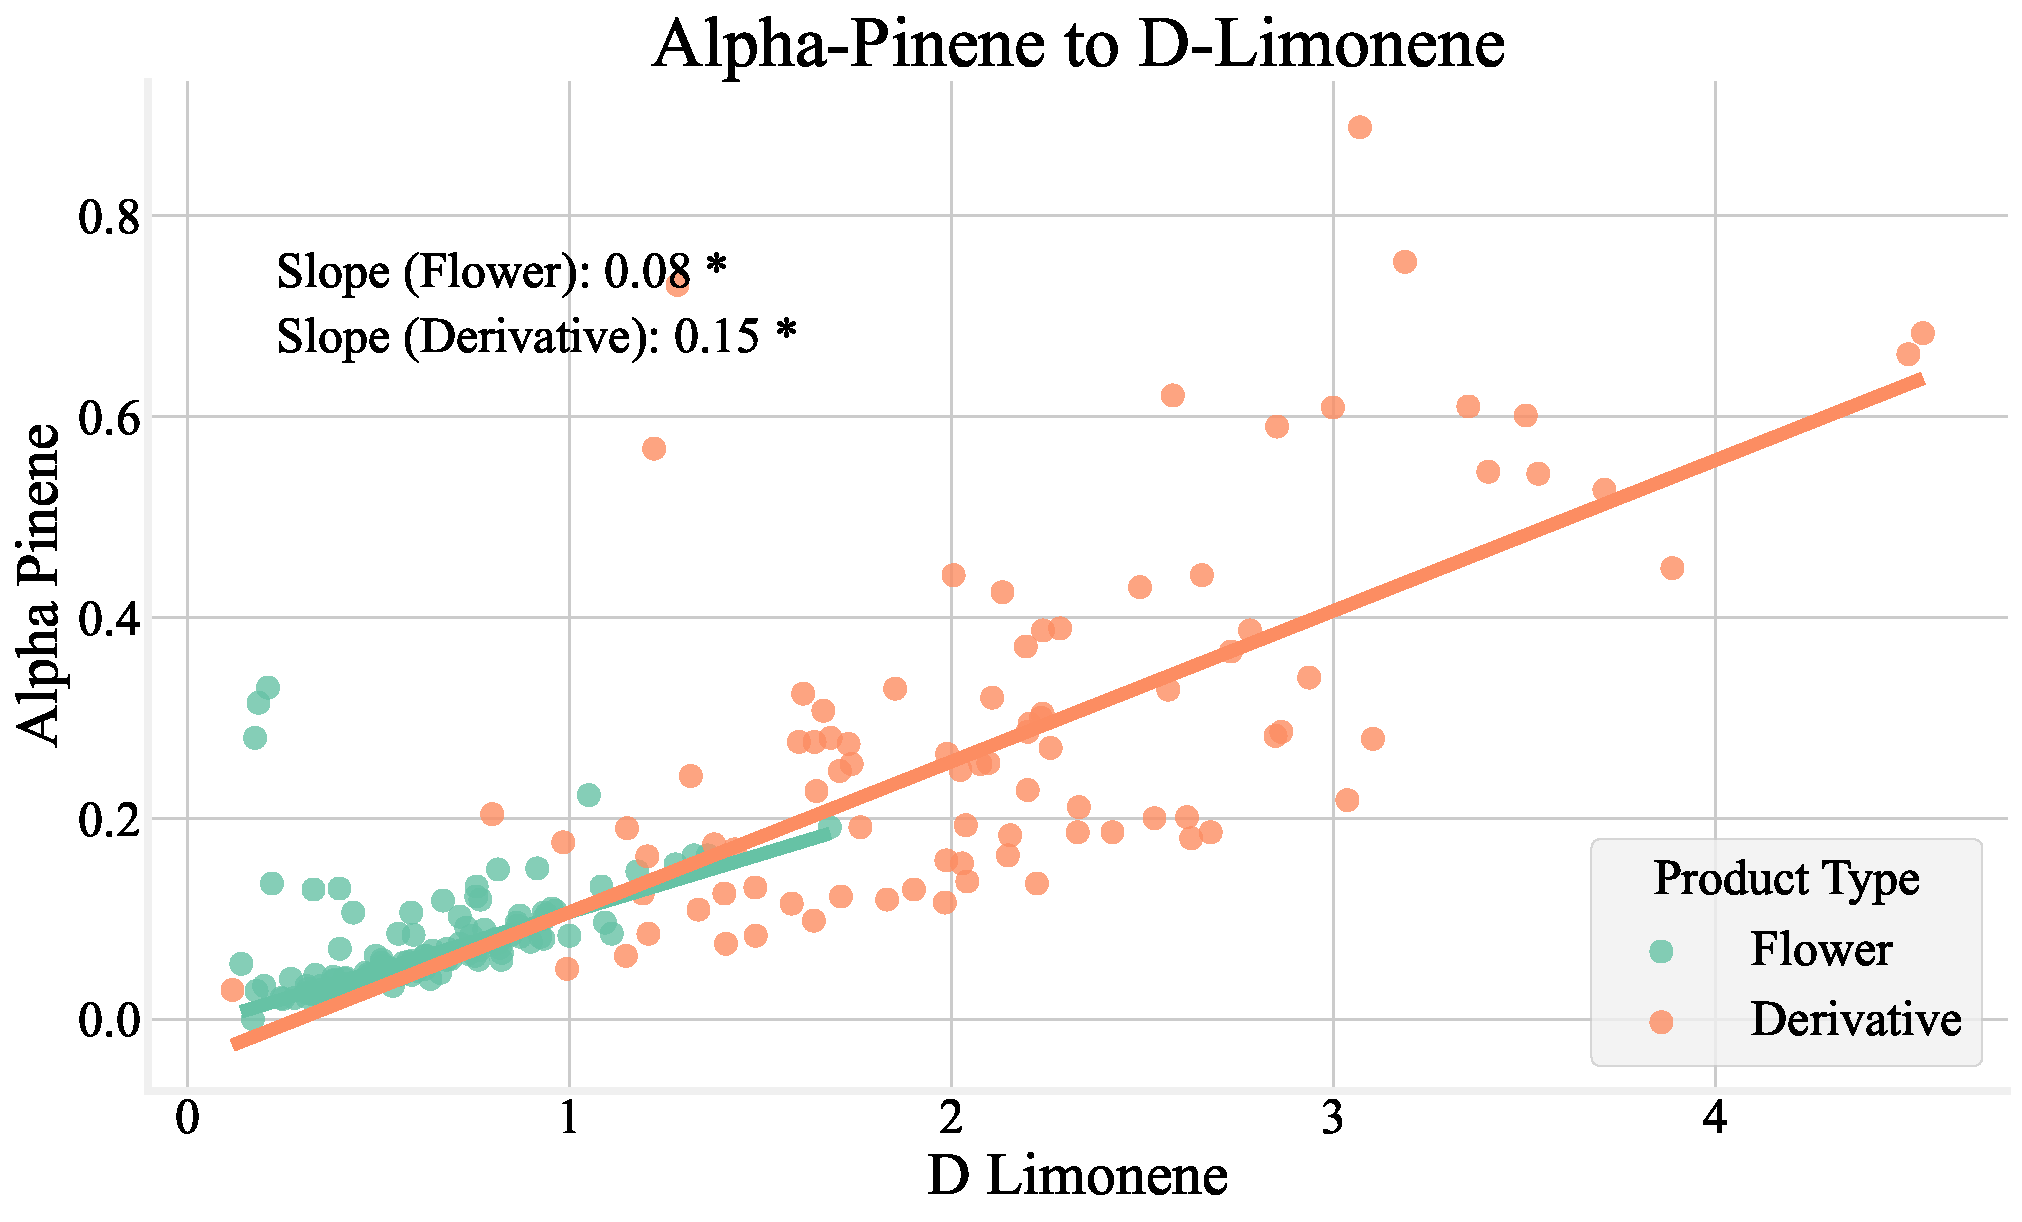
\includegraphics[width=\linewidth]{figures/alpha-pinene-to-d-limonene.pdf}

\vspace{2\baselineskip}

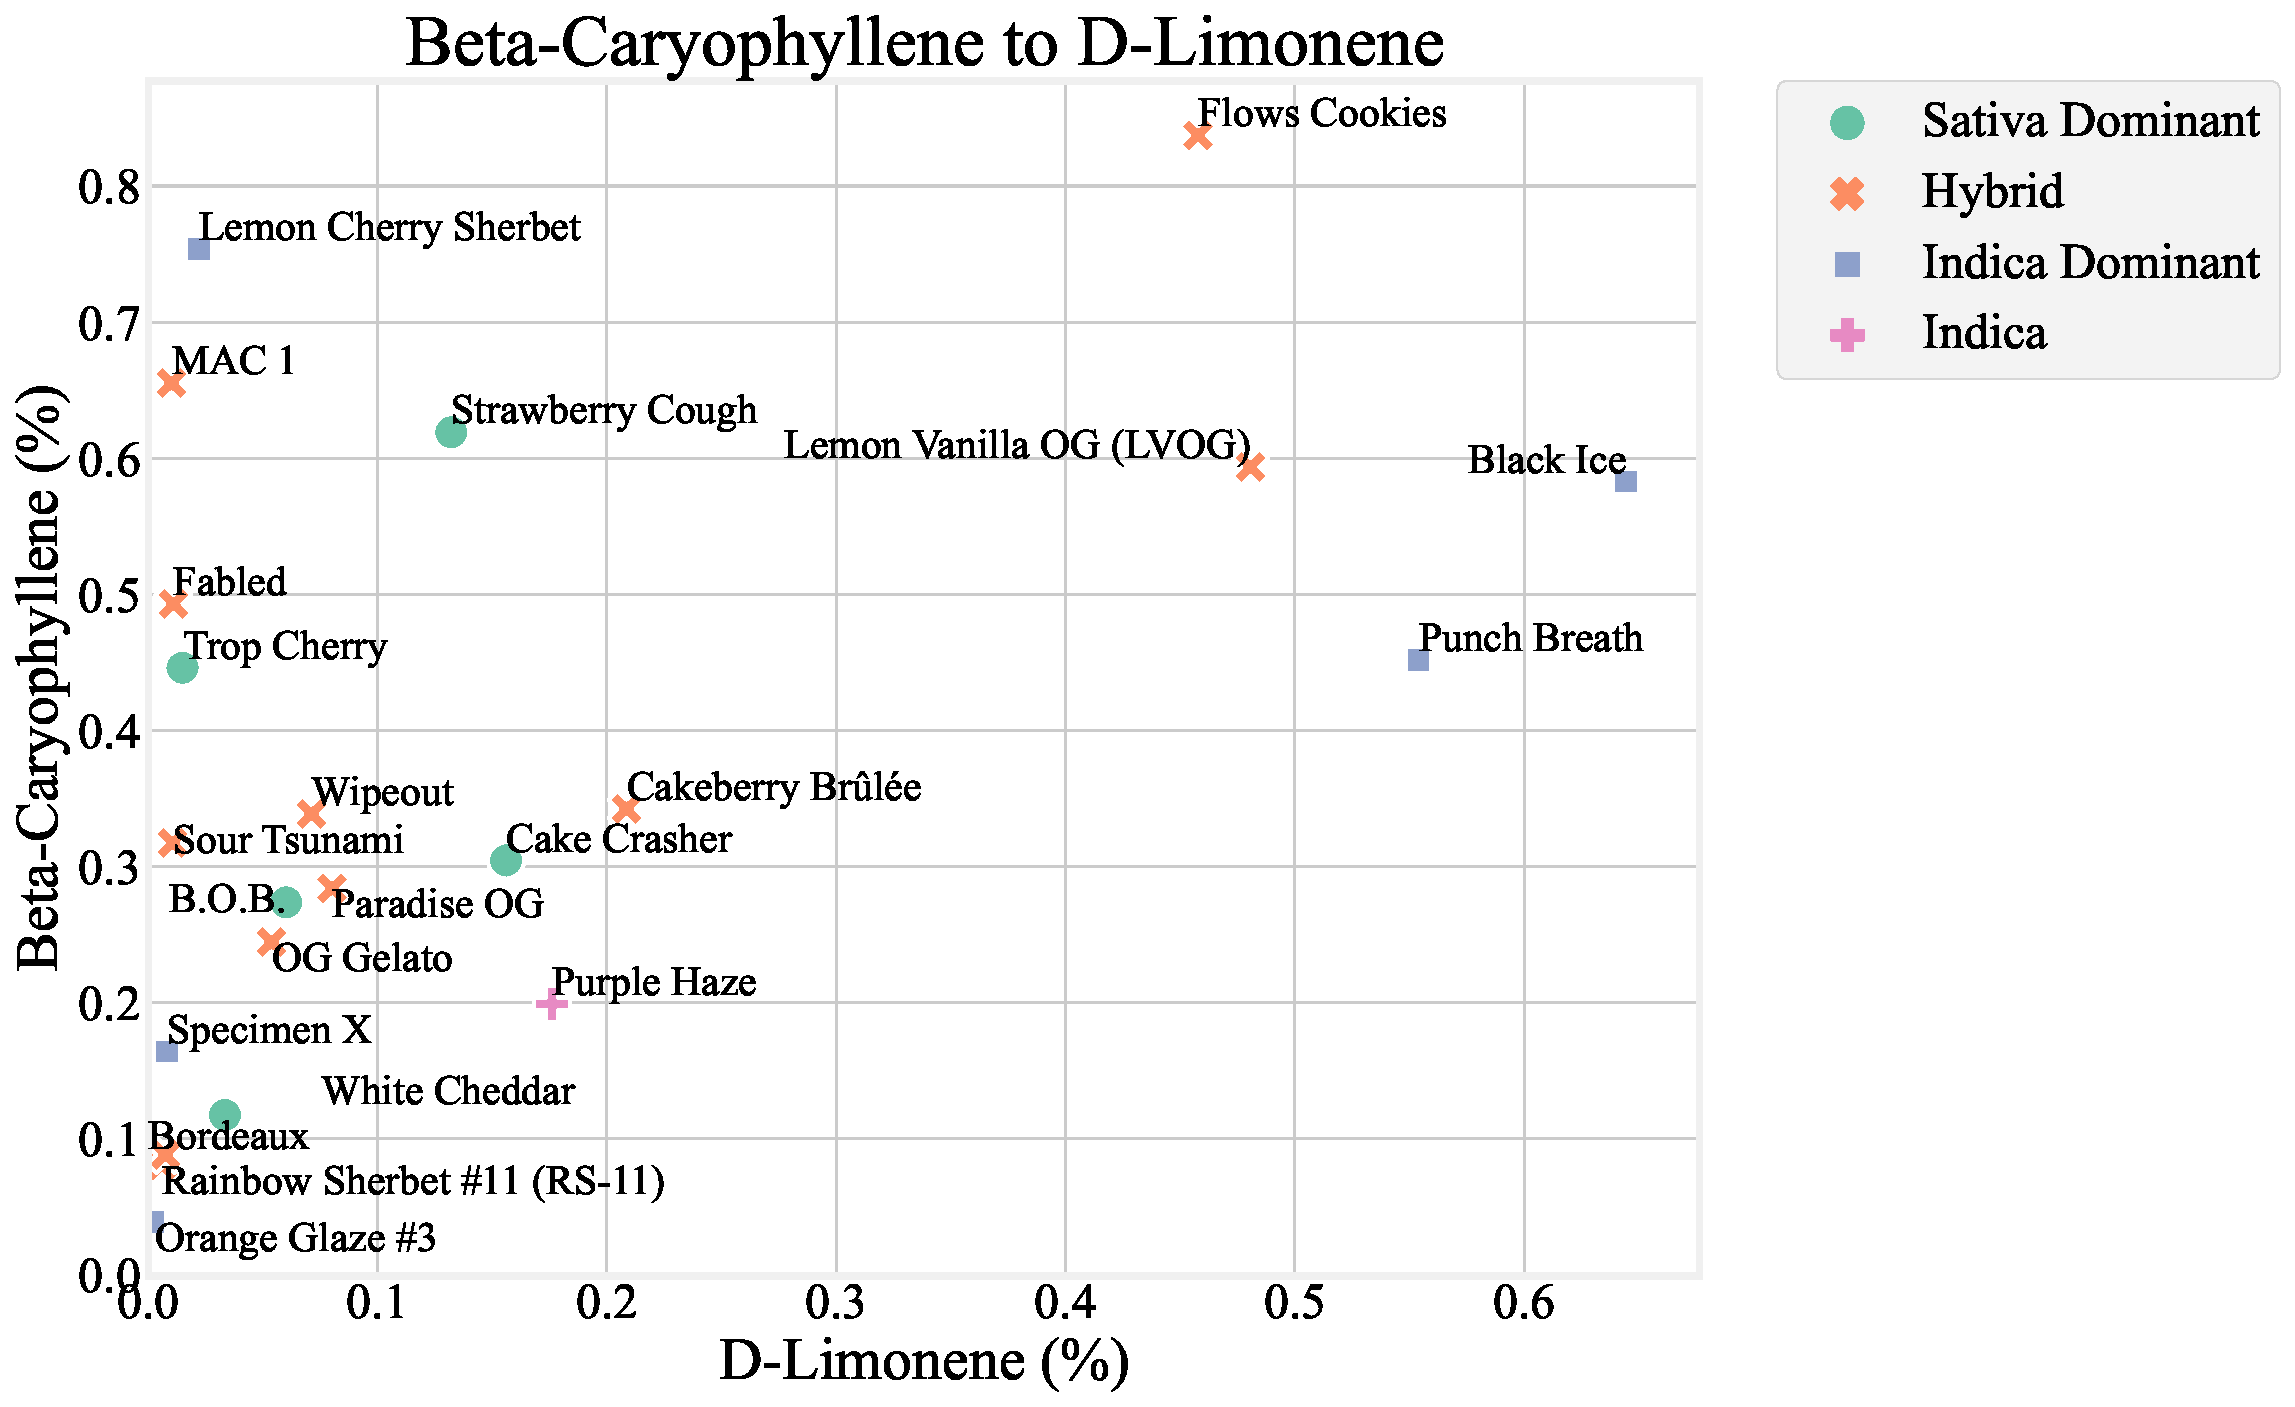
\includegraphics[width=\linewidth]{figures/beta-caryophyllene-to-d-limonene.pdf}

\vspace{2\baselineskip}

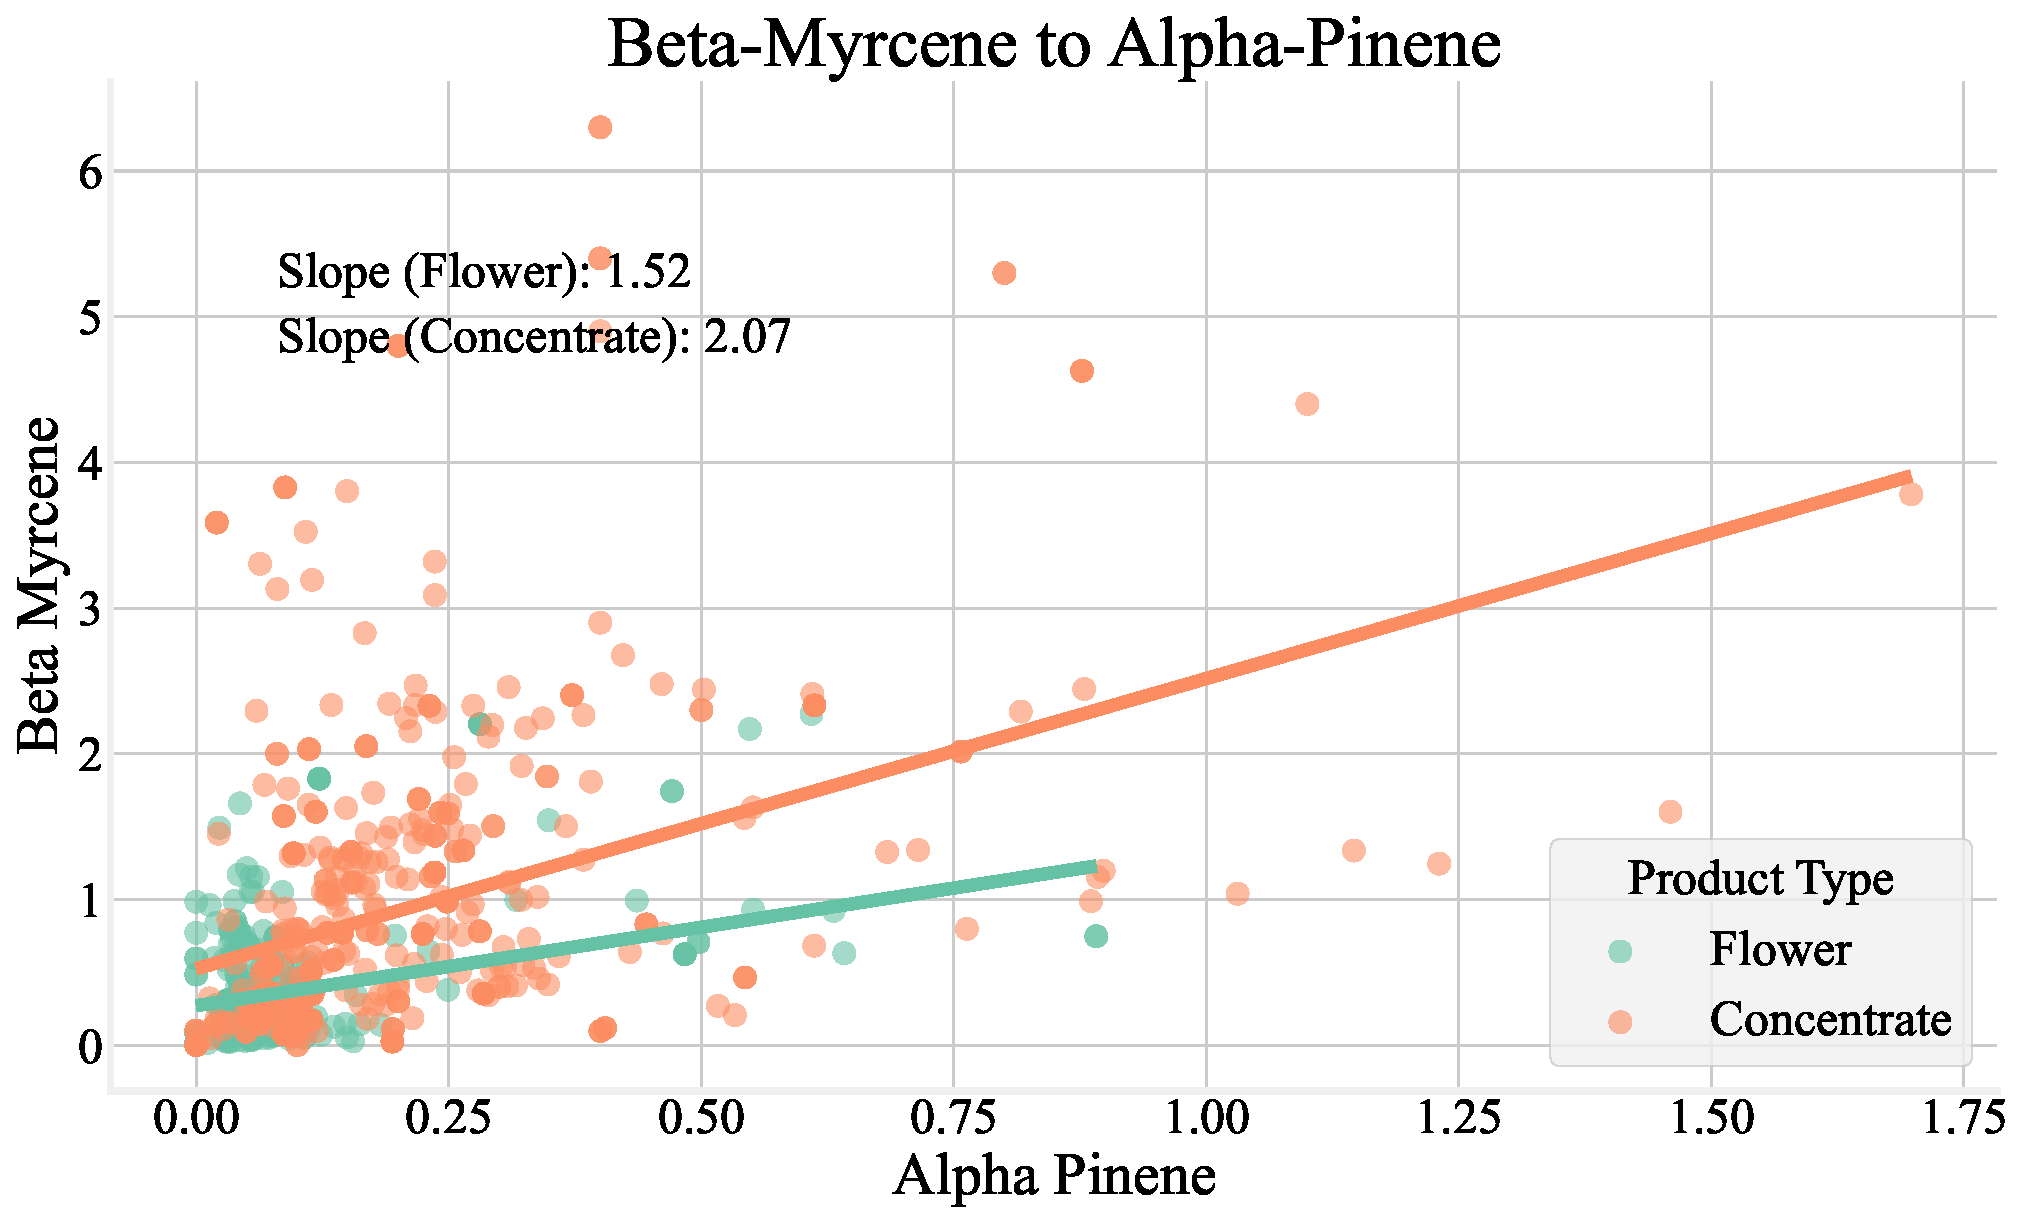
\includegraphics[width=\linewidth]{figures/beta-myrcene-to-alpha-pinene.pdf}

%\end{multicols}

\vspace{2\baselineskip}

% PCA
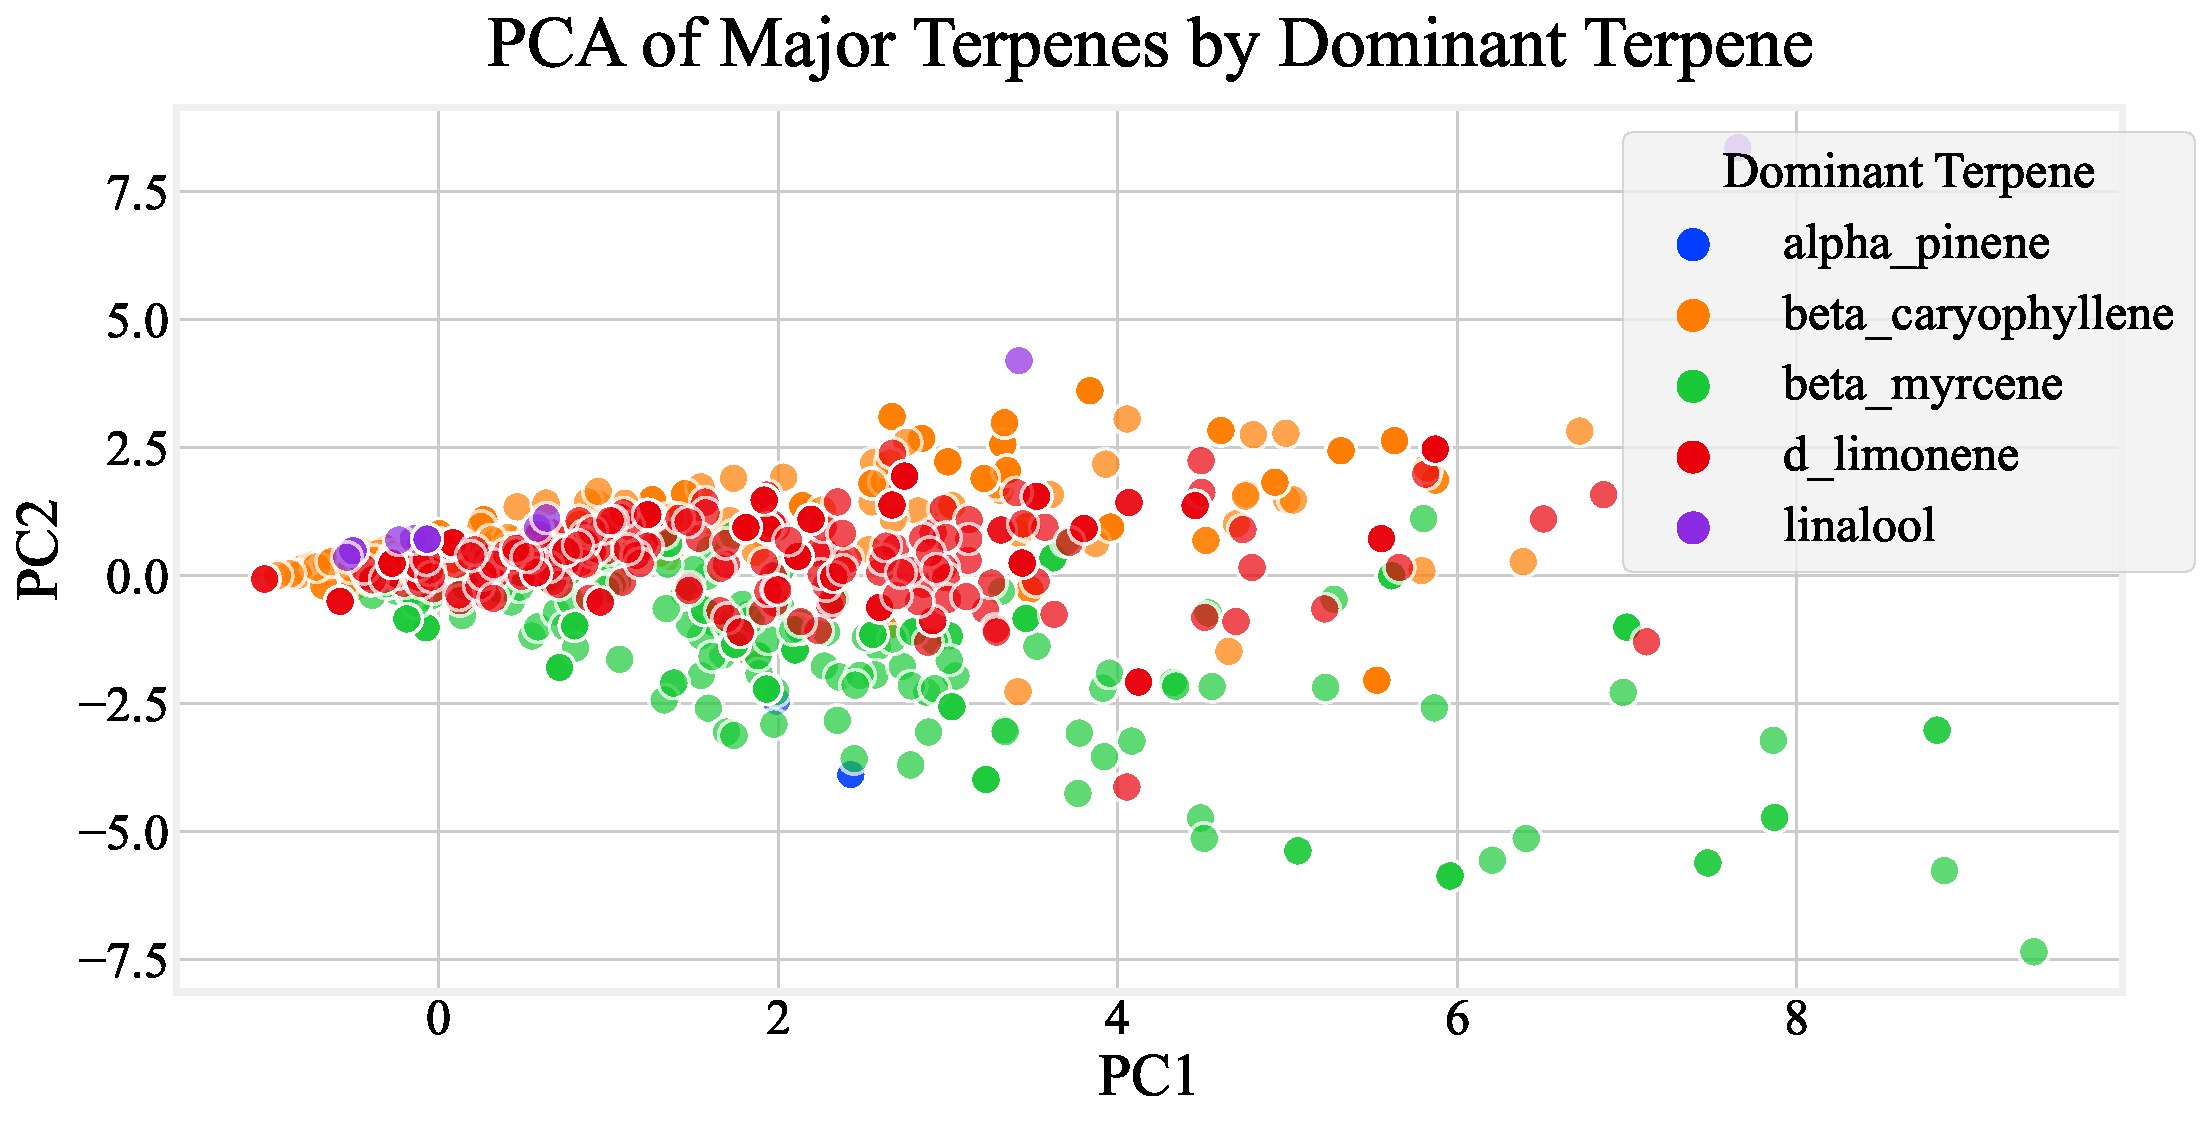
\includegraphics[width=\linewidth]{figures/pca-dominant-terpenes.pdf}


%---------------------------------%
% References
%---------------------------------%
%\newpage
%\nocite{*}
%\bibliography{references}
\thispagestyle{regular}

%---------------------------------%
% End of the Body
%---------------------------------%
\thispagestyle{regular}
\end{document}
